\documentclass[twoside]{book}

% Packages required by doxygen
\usepackage{fixltx2e}
\usepackage{calc}
\usepackage{doxygen}
\usepackage[export]{adjustbox} % also loads graphicx
\usepackage{graphicx}
\usepackage[utf8]{inputenc}
\usepackage{makeidx}
\usepackage{multicol}
\usepackage{multirow}
\PassOptionsToPackage{warn}{textcomp}
\usepackage{textcomp}
\usepackage[nointegrals]{wasysym}
\usepackage[table]{xcolor}

% Font selection
\usepackage[T1]{fontenc}
\usepackage[scaled=.90]{helvet}
\usepackage{courier}
\usepackage{amssymb}
\usepackage{sectsty}
\renewcommand{\familydefault}{\sfdefault}
\allsectionsfont{%
  \fontseries{bc}\selectfont%
  \color{darkgray}%
}
\renewcommand{\DoxyLabelFont}{%
  \fontseries{bc}\selectfont%
  \color{darkgray}%
}
\newcommand{\+}{\discretionary{\mbox{\scriptsize$\hookleftarrow$}}{}{}}

% Page & text layout
\usepackage{geometry}
\geometry{%
  a4paper,%
  top=2.5cm,%
  bottom=2.5cm,%
  left=2.5cm,%
  right=2.5cm%
}
\tolerance=750
\hfuzz=15pt
\hbadness=750
\setlength{\emergencystretch}{15pt}
\setlength{\parindent}{0cm}
\setlength{\parskip}{3ex plus 2ex minus 2ex}
\makeatletter
\renewcommand{\paragraph}{%
  \@startsection{paragraph}{4}{0ex}{-1.0ex}{1.0ex}{%
    \normalfont\normalsize\bfseries\SS@parafont%
  }%
}
\renewcommand{\subparagraph}{%
  \@startsection{subparagraph}{5}{0ex}{-1.0ex}{1.0ex}{%
    \normalfont\normalsize\bfseries\SS@subparafont%
  }%
}
\makeatother

% Headers & footers
\usepackage{fancyhdr}
\pagestyle{fancyplain}
\fancyhead[LE]{\fancyplain{}{\bfseries\thepage}}
\fancyhead[CE]{\fancyplain{}{}}
\fancyhead[RE]{\fancyplain{}{\bfseries\leftmark}}
\fancyhead[LO]{\fancyplain{}{\bfseries\rightmark}}
\fancyhead[CO]{\fancyplain{}{}}
\fancyhead[RO]{\fancyplain{}{\bfseries\thepage}}
\fancyfoot[LE]{\fancyplain{}{}}
\fancyfoot[CE]{\fancyplain{}{}}
\fancyfoot[RE]{\fancyplain{}{\bfseries\scriptsize Generated by Doxygen }}
\fancyfoot[LO]{\fancyplain{}{\bfseries\scriptsize Generated by Doxygen }}
\fancyfoot[CO]{\fancyplain{}{}}
\fancyfoot[RO]{\fancyplain{}{}}
\renewcommand{\footrulewidth}{0.4pt}
\renewcommand{\chaptermark}[1]{%
  \markboth{#1}{}%
}
\renewcommand{\sectionmark}[1]{%
  \markright{\thesection\ #1}%
}

% Indices & bibliography
\usepackage{natbib}
\usepackage[titles]{tocloft}
\setcounter{tocdepth}{3}
\setcounter{secnumdepth}{5}
\makeindex

% Custom commands
\newcommand{\clearemptydoublepage}{%
  \newpage{\pagestyle{empty}\cleardoublepage}%
}

\usepackage{caption}
\captionsetup{labelsep=space,justification=centering,font={bf},singlelinecheck=off,skip=4pt,position=top}

%===== C O N T E N T S =====

\begin{document}

% Titlepage & ToC
\pagenumbering{alph}
\begin{titlepage}
\vspace*{7cm}
\begin{center}%
{\Large S\+H1106 }\\
\vspace*{1cm}
{\large Generated by Doxygen 1.8.13}\\
\end{center}
\end{titlepage}
\clearemptydoublepage
\pagenumbering{roman}
\tableofcontents
\clearemptydoublepage
\pagenumbering{arabic}

%--- Begin generated contents ---
\chapter{Arduino Driver for S\+H1106 O\+L\+ED Controller}
\label{index}



{\bfseries Author}\+: Noè Archimede Pezzoli ({\tt noearchimede@gmail.\+com})~\newline
 {\bfseries Date}\+: 4/2018~\newline
 



The S\+H1106 library provides useful functions to write text and images to a display controlled by an S\+H1106 O\+L\+ED driver storing as little data as possible on the microcontroller (no buffer is required).

Currently this library only supports I2C interface, but other interfaces can be easily added (only a little derived class needs to be implemented for every new interface). Other display controllers may be made compatible as well.

The library is structured as follows\+:
\begin{DoxyEnumerate}
\item User classes\+: {\itshape \doxyref{Label}{p.}{class_label}} and {\itshape \doxyref{Image}{p.}{class_image}}
\item S\+H1106 driver class\+: {\itshape \doxyref{S\+H1106\+\_\+driver}{p.}{class_s_h1106__driver}}
\item S\+H1106 interface classes\+: {\itshape S\+H1106\+\_\+interfaces} -\/$>$ {\itshape \doxyref{S\+H1106\+\_\+\+I2C}{p.}{class_s_h1106___i2_c}}, ...
\end{DoxyEnumerate}





The {\itshape \doxyref{Label}{p.}{class_label}} class provides the ability to write any A\+S\+C\+II character and some other symbols in a proportional width font (as opposed to monospaced font), quite small but well readable. The class automatically adds newlines to the printed text taking care not to break words. Calling

{\ttfamily [\doxyref{Label}{p.}{class_label}\+:\+:]print(\char`\"{}\+Lorem ipsum dolor sit amet, consectetuer adipiscing elit. Aenean commodo ligula eget dolor. Aenean massa. Cum sociis natoque penatibus et magnis dis parturient montes, nascetur ridiculus mus. Donec quam felis,\char`\"{});}

produces the following printed result\+: 
\begin{DoxyCode}
Lorem ipsum dolor sit amet,
consectetuer adipiscing elit
Aenean commodo ligula eget
dolor. Aenean massa. Cum
sociis natoque penatibus et
magnis dis parturient
montes, nascetur ridiculus
mus. Donec quam felis,
\end{DoxyCode}
 It is possible to print text strings and literals stored either in R\+AM or in Flash memory, integer and floating point numbers (optionally aligning numbers on different lines), tabs, some control and other special characters, and any custom symbol saved as plain arrays of bytes. 



The {\itshape \doxyref{Image}{p.}{class_image}} class provides a simple interface to print bitmaps stored in byte arrays. The arrays are print in the order showed in this example, were an image of 5 pixels width and 4 pages height (5 x 32 pixels) is printed. 
\begin{DoxyCode}
03-07-11-15-19 -> page 0 (1 page is 8 pixels high)
02-06-10-14-18 -> page 1
01-05-09-13-17 -> page 2
00-04-08-12-16 -> page 3
|  |  |  |  |  
v  v  v  v  v  
0  1  2  3  4 columns (each 1 pixel wide)
\end{DoxyCode}




For more information please refer to the documentation in comments, wich can be extracted with Doxygen and is available {\tt Here}, and to the example program. 
\chapter{Hierarchical Index}
\section{Class Hierarchy}
This inheritance list is sorted roughly, but not completely, alphabetically\+:\begin{DoxyCompactList}
\item \contentsline{section}{Image}{\pageref{class_image}}{}
\item \contentsline{section}{Label}{\pageref{class_label}}{}
\item \contentsline{section}{Page\+Font}{\pageref{struct_page_font}}{}
\item \contentsline{section}{S\+H1106\+\_\+driver}{\pageref{class_s_h1106__driver}}{}
\item \contentsline{section}{S\+H1106\+\_\+interface}{\pageref{class_s_h1106__interface}}{}
\begin{DoxyCompactList}
\item \contentsline{section}{S\+H1106\+\_\+\+I2C}{\pageref{class_s_h1106___i2_c}}{}
\end{DoxyCompactList}
\end{DoxyCompactList}

\chapter{Class Index}
\section{Class List}
Here are the classes, structs, unions and interfaces with brief descriptions\+:\begin{DoxyCompactList}
\item\contentsline{section}{\textbf{ Image} \\*\doxyref{Image}{p.}{class_image} drawing class }{\pageref{class_image}}{}
\item\contentsline{section}{\textbf{ Label} \\*Text printing class }{\pageref{class_label}}{}
\item\contentsline{section}{\textbf{ Page\+Font} \\*Definition of a set of characters designed to fit an 8-\/bit page }{\pageref{struct_page_font}}{}
\item\contentsline{section}{\textbf{ S\+H1106\+\_\+driver} \\*S\+H1106 O\+L\+ED controller communication management }{\pageref{class_s_h1106__driver}}{}
\item\contentsline{section}{\textbf{ S\+H1106\+\_\+\+I2C} \\*I2C interface implementation class This class allows to communicate with an S\+H1106 through i2c interface }{\pageref{class_s_h1106___i2_c}}{}
\item\contentsline{section}{\textbf{ S\+H1106\+\_\+interface} \\*Abstract class to describe any interface to communicate with S\+H1106 }{\pageref{class_s_h1106__interface}}{}
\end{DoxyCompactList}

\chapter{Class Documentation}
\section{Image Class Reference}
\label{class_image}\index{Image@{Image}}


\doxyref{Image}{p.}{class_image} drawing class.  




{\ttfamily \#include $<$Image.\+hpp$>$}

\subsection*{Public Member Functions}
\begin{DoxyCompactItemize}
\item 
\textbf{ Image} (\textbf{ S\+H1106\+\_\+driver} \&display, uint8\+\_\+t width, uint8\+\_\+t height, uint8\+\_\+t start\+Column, uint8\+\_\+t start\+Page)
\begin{DoxyCompactList}\small\item\em Consturctor -\/ provides image size and position. \end{DoxyCompactList}\item 
void \textbf{ draw} (const uint8\+\_\+t image[$\,$], bool progmem)
\begin{DoxyCompactList}\small\item\em Draw an image in the label. \end{DoxyCompactList}\item 
void \textbf{ clear} ()
\begin{DoxyCompactList}\small\item\em Clear the frame. \end{DoxyCompactList}\item 
void \textbf{ fill} (uint8\+\_\+t data=0x00)
\begin{DoxyCompactList}\small\item\em fill the frame with a given single byte \end{DoxyCompactList}\item 
void \textbf{ fill} (uint8\+\_\+t $\ast$pattern, uint8\+\_\+t length)
\begin{DoxyCompactList}\small\item\em fill the image with a given pattern \end{DoxyCompactList}\end{DoxyCompactItemize}


\subsection{Detailed Description}
\doxyref{Image}{p.}{class_image} drawing class. 

Tha \doxyref{Image}{p.}{class_image} class allows to write a bitmap image on a given area of the screen. The frame can have any size in width, but it\textquotesingle{}s height must be a multiple of 8 as well as its y position because it needs to fit an integer number of pages.

The image must be represented as an unidimensional array of bytes. One byte represents a vertical 8-\/pixel line whose top pixel is the most significant bit of the pixel. The byte sequence procedes from left to right and then from top to bottom.

\begin{DoxyWarning}{Warning}
The image array must have enough bytes to fill the entire frame, i.\+e. to a 20 columns x 24 rows (i.\+e. 3 pages) an array of (at least) 60 bytes must be passed. 
\end{DoxyWarning}


Definition at line 27 of file Image.\+hpp.



\subsection{Constructor \& Destructor Documentation}
\mbox{\label{class_image_a36c4165842076d529e87a7f10e583f9f}} 
\index{Image@{Image}!Image@{Image}}
\index{Image@{Image}!Image@{Image}}
\subsubsection{Image()}
{\footnotesize\ttfamily Image\+::\+Image (\begin{DoxyParamCaption}\item[{\textbf{ S\+H1106\+\_\+driver} \&}]{display,  }\item[{uint8\+\_\+t}]{width,  }\item[{uint8\+\_\+t}]{height,  }\item[{uint8\+\_\+t}]{start\+Column,  }\item[{uint8\+\_\+t}]{start\+Page }\end{DoxyParamCaption})}



Consturctor -\/ provides image size and position. 



Definition at line 7 of file Image.\+cpp.



\subsection{Member Function Documentation}
\mbox{\label{class_image_aa0db6a748a2d7039d2f1a312f5234744}} 
\index{Image@{Image}!draw@{draw}}
\index{draw@{draw}!Image@{Image}}
\subsubsection{draw()}
{\footnotesize\ttfamily void Image\+::draw (\begin{DoxyParamCaption}\item[{const uint8\+\_\+t}]{image[$\,$],  }\item[{bool}]{progmem }\end{DoxyParamCaption})}



Draw an image in the label. 

The size of the image must match the frame size. If it doesn\textquotesingle{}t the behaviour is not defined. 
\begin{DoxyParams}{Parameters}
{\em progmem} & true if the array is stored in P\+R\+O\+G\+M\+EM, false if it is in R\+AM. \\
\hline
\end{DoxyParams}


Definition at line 14 of file Image.\+cpp.

\mbox{\label{class_image_a3a233515eb3a5f83917dc634c778db5a}} 
\index{Image@{Image}!clear@{clear}}
\index{clear@{clear}!Image@{Image}}
\subsubsection{clear()}
{\footnotesize\ttfamily void Image\+::clear (\begin{DoxyParamCaption}{ }\end{DoxyParamCaption})}



Clear the frame. 

The cursor will be moved to (0,0) 

Definition at line 25 of file Image.\+cpp.

\mbox{\label{class_image_a2d97588a695f36d550029ee9bfa4cb7a}} 
\index{Image@{Image}!fill@{fill}}
\index{fill@{fill}!Image@{Image}}
\subsubsection{fill()\hspace{0.1cm}{\footnotesize\ttfamily [1/2]}}
{\footnotesize\ttfamily void Image\+::fill (\begin{DoxyParamCaption}\item[{uint8\+\_\+t}]{data = {\ttfamily 0x00} }\end{DoxyParamCaption})}



fill the frame with a given single byte 


\begin{DoxyParams}{Parameters}
{\em data} & the byte that will be repeatedly printed. \\
\hline
\end{DoxyParams}


Definition at line 30 of file Image.\+cpp.

\mbox{\label{class_image_ac46c2fcd8a030c06e3fe76632117ea46}} 
\index{Image@{Image}!fill@{fill}}
\index{fill@{fill}!Image@{Image}}
\subsubsection{fill()\hspace{0.1cm}{\footnotesize\ttfamily [2/2]}}
{\footnotesize\ttfamily void Image\+::fill (\begin{DoxyParamCaption}\item[{uint8\+\_\+t $\ast$}]{pattern,  }\item[{uint8\+\_\+t}]{length }\end{DoxyParamCaption})}



fill the image with a given pattern 


\begin{DoxyParams}{Parameters}
{\em pattern} & this array will be repeatedly print to fill the frame \\
\hline
{\em length} & length of the pattern array \\
\hline
\end{DoxyParams}


Definition at line 34 of file Image.\+cpp.



The documentation for this class was generated from the following files\+:\begin{DoxyCompactItemize}
\item 
/\+Users/noe/\+Documents/\+Robot/\+Librerie/\+S\+H1106/\+S\+H1106/Image.\+hpp\item 
/\+Users/noe/\+Documents/\+Robot/\+Librerie/\+S\+H1106/\+S\+H1106/Image.\+cpp\end{DoxyCompactItemize}

\section{Label Class Reference}
\label{class_label}\index{Label@{Label}}


Text printing class.  




{\ttfamily \#include $<$Label.\+hpp$>$}

\subsection*{Public Member Functions}
\begin{DoxyCompactItemize}
\item 
\textbf{ Label} (\textbf{ S\+H1106\+\_\+driver} \&display, uint8\+\_\+t width, uint8\+\_\+t height, uint8\+\_\+t start\+Column, uint8\+\_\+t start\+Page)
\begin{DoxyCompactList}\small\item\em Consturctor -\/ provides label size and position. \end{DoxyCompactList}\item 
bool \textbf{ print} (const char $\ast$text)
\begin{DoxyCompactList}\small\item\em Print a N\+U\+L\+L-\/\+T\+E\+R\+M\+I\+N\+A\+T\+ED string literal or char array on the screen. \end{DoxyCompactList}\item 
bool \textbf{ print} (const char $\ast$text, bool progmem)
\begin{DoxyCompactList}\small\item\em Print a N\+U\+L\+L\+\_\+terminated string in a given memory space (P\+R\+O\+G\+M\+E\+M/\+R\+AM) \end{DoxyCompactList}\item 
bool \textbf{ print} (const \+\_\+\+\_\+\+Flash\+String\+Helper $\ast$text)
\begin{DoxyCompactList}\small\item\em Print a string literal put inside the {\ttfamily F()} macro. \end{DoxyCompactList}\item 
bool \textbf{ print} (char c)
\begin{DoxyCompactList}\small\item\em Print a single A\+S\+C\+II character. \end{DoxyCompactList}\item 
bool \textbf{ print} (unsigned char n, uint8\+\_\+t base=10, uint8\+\_\+t min\+Width=0)
\begin{DoxyCompactList}\small\item\em Print an integer number. \end{DoxyCompactList}\item 
bool \textbf{ print} (char n, uint8\+\_\+t base, uint8\+\_\+t min\+Width=0)
\begin{DoxyCompactList}\small\item\em See above. \end{DoxyCompactList}\item 
bool \textbf{ print} (unsigned int n, uint8\+\_\+t base=10, uint8\+\_\+t min\+Width=0)
\begin{DoxyCompactList}\small\item\em See above. \end{DoxyCompactList}\item 
bool \textbf{ print} (int n, uint8\+\_\+t base=10, uint8\+\_\+t min\+Width=0)
\begin{DoxyCompactList}\small\item\em See above. \end{DoxyCompactList}\item 
bool \textbf{ print} (unsigned long n, uint8\+\_\+t base=10, uint8\+\_\+t min\+Width=0)
\begin{DoxyCompactList}\small\item\em See above. \end{DoxyCompactList}\item 
bool \textbf{ print} (long n, uint8\+\_\+t base=10, uint8\+\_\+t min\+Width=0)
\begin{DoxyCompactList}\small\item\em See aboveß \end{DoxyCompactList}\item 
bool \textbf{ print} (float n, uint8\+\_\+t fract\+Digits=2, uint8\+\_\+t min\+Int\+Digits=0)
\begin{DoxyCompactList}\small\item\em Print a floating point number. \end{DoxyCompactList}\item 
bool \textbf{ print} (double n, uint8\+\_\+t fract\+Digits=2, uint8\+\_\+t min\+Int\+Digits=0)
\begin{DoxyCompactList}\small\item\em same as above \end{DoxyCompactList}\item 
bool \textbf{ print} (const char text[$\,$], uint16\+\_\+t length, bool progmem)
\begin{DoxyCompactList}\small\item\em Print a char array of given lenght on the screen. \end{DoxyCompactList}\item 
void \textbf{ clear} ()
\begin{DoxyCompactList}\small\item\em Clear the label. \end{DoxyCompactList}\item 
bool \textbf{ tab} (uint8\+\_\+t anchor=0)
\begin{DoxyCompactList}\small\item\em Write a tab. \end{DoxyCompactList}\item 
bool \textbf{ newline} ()
\begin{DoxyCompactList}\small\item\em Go to the next line. \end{DoxyCompactList}\item 
bool \textbf{ carriage\+Return\+Clear} ()
\begin{DoxyCompactList}\small\item\em Go to the beginning of current line and clear line. \end{DoxyCompactList}\item 
bool \textbf{ space} ()
\begin{DoxyCompactList}\small\item\em Write a space. \end{DoxyCompactList}\item 
void \textbf{ fill} (uint8\+\_\+t data=0x00, uint8\+\_\+t begin\+Col=0, uint8\+\_\+t begin\+Pag=0, uint8\+\_\+t end\+Col=0x\+F\+F, uint8\+\_\+t end\+Pag=0x\+F\+F)
\begin{DoxyCompactList}\small\item\em Write a single byte on a given part of the label. \end{DoxyCompactList}\item 
bool \textbf{ write\+Array} (const uint8\+\_\+t data[$\,$], uint8\+\_\+t length)
\begin{DoxyCompactList}\small\item\em Draw a number of consecutive bytes on a page as if it were a character. \end{DoxyCompactList}\item 
bool \textbf{ set\+Cursor} (uint8\+\_\+t column, uint8\+\_\+t page)
\begin{DoxyCompactList}\small\item\em Move the cursor to a given location. \end{DoxyCompactList}\item 
void \textbf{ get\+Cursor} (uint8\+\_\+t \&column, uint8\+\_\+t \&page)
\begin{DoxyCompactList}\small\item\em Get the current cursor position. \end{DoxyCompactList}\item 
uint8\+\_\+t \textbf{ available\+Columns} ()
\begin{DoxyCompactList}\small\item\em Get the remaining space on current line. \end{DoxyCompactList}\item 
uint8\+\_\+t \textbf{ available\+Pages} ()
\begin{DoxyCompactList}\small\item\em Get the number of available pages under the cursor. \end{DoxyCompactList}\item 
void \textbf{ get\+Size} (uint8\+\_\+t \&columns, uint8\+\_\+t \&pages)
\begin{DoxyCompactList}\small\item\em get the size of the label \end{DoxyCompactList}\item 
void \textbf{ set\+Infinite} (bool enable, bool empty\+Line)
\begin{DoxyCompactList}\small\item\em Set the cursor to use the first line as the one after the last. \end{DoxyCompactList}\end{DoxyCompactItemize}
\subsection*{Friends}
\begin{DoxyCompactItemize}
\item 
\mbox{\label{class_label_a9591eb6f6543f40292912e27b74f4d27}} 
class {\bfseries Cursor}
\end{DoxyCompactItemize}


\subsection{Detailed Description}
Text printing class. 

The \doxyref{Label}{p.}{class_label} class allows to write any A\+S\+C\+II character plus some other symbols in a frame of a given size set by the user in the constructor. There is no limit to the amount of labels on a single display, as long as there is enough free space. In case of overlapping of two displays (or other drawing entities) the most recently active will partially or completely overwrite the other one.

The text is always written in a single page, so that the microcontroller doesn\textquotesingle{}t need to hold a copy of the dysplay R\+AM (all writing operations are to be performed on whole pages, so if the text fills exactly one page there is no need to preserve (thus know) some content when overwriting). Since there isn\textquotesingle{}t much available space in a single 8-\/bit page, the text size and font style are fixed.

The text is printed using the {\ttfamily \doxyref{print()}{p.}{class_label_a2ad62b03233003c1e94338f676638564}} function, wich takes either a string literal or a N\+U\+L\+L-\/terminated string either a char array and its lenght as a second parameter. The print function allows to write A\+S\+C\+II printable characters (i.\+e. A\+S\+C\+II characters 0x20 to 0x7E) as well as some special characters, obtained by writing the following two character sequences. The backslash \textquotesingle{}\textbackslash{}\textquotesingle{} is used as escape character. Unless the user uses raw string literals, the escape character must be written twice to pass it to the class as a single backslash is interpreted by the compiler\+: e.\+g. write \char`\"{}\textbackslash{}\textbackslash{}$^\wedge$\char`\"{} to get the escape sequence \char`\"{}\textbackslash{}$^\wedge$\char`\"{} (up arrow).

\tabulinesep=1mm
\begin{longtabu} spread 0pt [c]{*{2}{|X[-1]}|}
\hline
\rowcolor{\tableheadbgcolor}\textbf{ A\+S\+C\+II control characters }&\textbf{ }\\\cline{1-2}
\endfirsthead
\hline
\endfoot
\hline
\rowcolor{\tableheadbgcolor}\textbf{ A\+S\+C\+II control characters }&\textbf{ }\\\cline{1-2}
\endhead
\textbackslash{}n &newline \\\cline{1-2}
\textbackslash{}t &tab \\\cline{1-2}
\textbackslash{}r &carriage return; clears current line \\\cline{1-2}
\end{longtabu}
\tabulinesep=1mm
\begin{longtabu} spread 0pt [c]{*{2}{|X[-1]}|}
\hline
\rowcolor{\tableheadbgcolor}\textbf{ Accents }&\textbf{ }\\\cline{1-2}
\endfirsthead
\hline
\endfoot
\hline
\rowcolor{\tableheadbgcolor}\textbf{ Accents }&\textbf{ }\\\cline{1-2}
\endhead
a{\ttfamily $<$td$>$ à $<$tr$>$$<$td$>$ e} &è \\\cline{1-2}
i{\ttfamily $<$td$>$ ì $<$tr$>$$<$td$>$ o} &ò \\\cline{1-2}
u` &ù \\\cline{1-2}
\end{longtabu}
\tabulinesep=1mm
\begin{longtabu} spread 0pt [c]{*{2}{|X[-1]}|}
\hline
\rowcolor{\tableheadbgcolor}\textbf{ Arrows }&\textbf{ }\\\cline{1-2}
\endfirsthead
\hline
\endfoot
\hline
\rowcolor{\tableheadbgcolor}\textbf{ Arrows }&\textbf{ }\\\cline{1-2}
\endhead
\textbackslash{}$^\wedge$ &UP \\\cline{1-2}
-\/$^\wedge$ &UP R\+I\+G\+HT \\\cline{1-2}
-\/$>$ &R\+I\+G\+HT \\\cline{1-2}
-\/v &D\+O\+WN R\+I\+G\+HT \\\cline{1-2}
&D\+O\+WN \\\cline{1-2}
v-\/ &D\+O\+WN L\+E\+FT \\\cline{1-2}
$<$-\/ &L\+E\+FT \\\cline{1-2}
$^\wedge$-\/ &UP L\+E\+FT \\\cline{1-2}
\end{longtabu}
{\itshape Note\+: up sign is a circumflex accent, down is a lower case \textquotesingle{}v\textquotesingle{}}

$\vert$ Digits at exponent position $\vert$$\vert$ $\vert$-\/-\/-\/-\/-\/-\/-\/-\/-\/-\/-\/-\/-\/-\/-\/-\/-\/-\/-\/-\/-\/-\/-\/-\/-\/-\/-\/-\/-\/-\/-\/-\/-\/-\/-\/-\/-\/-\/-\/-\/-\/-\/-\/-\/-\/-\/-\/-\/-\/-\/-\/-\/-\/-\/-\/-\/-\/-\/-\/-\/-\/-\/-\/-\/-\/---$\vert$ $\vert$ $^\wedge$x $\vert$ where x is any number from 0 to 9 $\vert$ $\vert$ $^\wedge$x$^\wedge$y $\vert$ two or more exponent digits need repeated escape sequences $\vert$

\tabulinesep=1mm
\begin{longtabu} spread 0pt [c]{*{2}{|X[-1]}|}
\hline
\rowcolor{\tableheadbgcolor}\textbf{ Other special characters }&\textbf{ }\\\cline{1-2}
\endfirsthead
\hline
\endfoot
\hline
\rowcolor{\tableheadbgcolor}\textbf{ Other special characters }&\textbf{ }\\\cline{1-2}
\endhead
$^\wedge$o &(lower case \textquotesingle{}o\textquotesingle{}) degree symbol \\\cline{1-2}
{\ttfamily } &copyright symbol © \\\cline{1-2}
\end{longtabu}


\tabulinesep=1mm
\begin{longtabu} spread 0pt [c]{*{2}{|X[-1]}|}
\hline
\rowcolor{\tableheadbgcolor}\textbf{ Escape character }&\textbf{ }\\\cline{1-2}
\endfirsthead
\hline
\endfoot
\hline
\rowcolor{\tableheadbgcolor}\textbf{ Escape character }&\textbf{ }\\\cline{1-2}
\endhead
\textbackslash{} &write it twice to print \\\cline{1-2}
\end{longtabu}


The escape character may be used within any of the above sequences to tell the writing function to print them as they are (e.\+g. \char`\"{}$^\wedge$o\char`\"{} prints \char`\"{}°\char`\"{} while \char`\"{}$^\wedge$\textbackslash{}o\char`\"{} prints \char`\"{}$^\wedge$o\char`\"{} and \char`\"{}$^\wedge$\textbackslash{}\textbackslash{}o\char`\"{} prints \char`\"{}$^\wedge$\textbackslash{}o\char`\"{}). 

Definition at line 88 of file Label.\+hpp.



\subsection{Constructor \& Destructor Documentation}
\mbox{\label{class_label_a9fa66219bff9119d44d056bc3e456d12}} 
\index{Label@{Label}!Label@{Label}}
\index{Label@{Label}!Label@{Label}}
\subsubsection{Label()}
{\footnotesize\ttfamily Label\+::\+Label (\begin{DoxyParamCaption}\item[{\textbf{ S\+H1106\+\_\+driver} \&}]{display,  }\item[{uint8\+\_\+t}]{width,  }\item[{uint8\+\_\+t}]{height,  }\item[{uint8\+\_\+t}]{start\+Column,  }\item[{uint8\+\_\+t}]{start\+Page }\end{DoxyParamCaption})}



Consturctor -\/ provides label size and position. 



Definition at line 6 of file Label.\+cpp.



\subsection{Member Function Documentation}
\mbox{\label{class_label_a2ad62b03233003c1e94338f676638564}} 
\index{Label@{Label}!print@{print}}
\index{print@{print}!Label@{Label}}
\subsubsection{print()\hspace{0.1cm}{\footnotesize\ttfamily [1/13]}}
{\footnotesize\ttfamily bool Label\+::print (\begin{DoxyParamCaption}\item[{const char $\ast$}]{text }\end{DoxyParamCaption})}



Print a N\+U\+L\+L-\/\+T\+E\+R\+M\+I\+N\+A\+T\+ED string literal or char array on the screen. 

The text is encoded in A\+S\+C\+II but can contain a number of special sequences, listed in the class description. It will be print starting from the current cursor position and will be cut at the end of the label. Words (sequences of characters beetween two spaces) will not be split between two lines, if there isn\textquotesingle{}t enough space for a word on the current line the cursor will automatically move to the next one, but spacing will not be influenced by the amount of free space at the end of the line.

\begin{DoxyWarning}{Warning}
The char array must end with a \textquotesingle{}\textbackslash{}0\textquotesingle{} (N\+U\+LL) character. \textquotesingle{}\textbackslash{}0\textquotesingle{} is automatically appended to string literals.
\end{DoxyWarning}

\begin{DoxyParams}{Parameters}
{\em text} & The char array containting the text to print \\
\hline
\end{DoxyParams}
\begin{DoxyReturn}{Returns}
{\ttfamily false} if there wasn\textquotesingle{}t space enough to print all the text. The function will write as many character as possible given the space available from current cursor position. 
\end{DoxyReturn}


Definition at line 27 of file Label.\+cpp.

\mbox{\label{class_label_a5714e7f4345db0886bd95ef71ad72d5a}} 
\index{Label@{Label}!print@{print}}
\index{print@{print}!Label@{Label}}
\subsubsection{print()\hspace{0.1cm}{\footnotesize\ttfamily [2/13]}}
{\footnotesize\ttfamily bool Label\+::print (\begin{DoxyParamCaption}\item[{const char $\ast$}]{text,  }\item[{bool}]{progmem }\end{DoxyParamCaption})}



Print a N\+U\+L\+L\+\_\+terminated string in a given memory space (P\+R\+O\+G\+M\+E\+M/\+R\+AM) 


\begin{DoxyParams}{Parameters}
{\em progmem} & {\ttfamily true} if the {\ttfamily text} is stored in P\+R\+O\+G\+M\+EM, {\ttfamily false} if it is in R\+AM \\
\hline
\end{DoxyParams}


Definition at line 44 of file Label.\+cpp.

\mbox{\label{class_label_a33ea2d99cc6554af1668f77371f93f19}} 
\index{Label@{Label}!print@{print}}
\index{print@{print}!Label@{Label}}
\subsubsection{print()\hspace{0.1cm}{\footnotesize\ttfamily [3/13]}}
{\footnotesize\ttfamily bool Label\+::print (\begin{DoxyParamCaption}\item[{const \+\_\+\+\_\+\+Flash\+String\+Helper $\ast$}]{text }\end{DoxyParamCaption})}



Print a string literal put inside the {\ttfamily F()} macro. 

Like {\ttfamily \doxyref{print(char)}{p.}{class_label_a24106d29becf8f26c8205b623ba63d08}} but works for string literals put in P\+R\+O\+G\+M\+EM by the {\ttfamily F()} macro. 

Definition at line 35 of file Label.\+cpp.

\mbox{\label{class_label_a24106d29becf8f26c8205b623ba63d08}} 
\index{Label@{Label}!print@{print}}
\index{print@{print}!Label@{Label}}
\subsubsection{print()\hspace{0.1cm}{\footnotesize\ttfamily [4/13]}}
{\footnotesize\ttfamily bool Label\+::print (\begin{DoxyParamCaption}\item[{char}]{c }\end{DoxyParamCaption})}



Print a single A\+S\+C\+II character. 



Definition at line 55 of file Label.\+cpp.

\mbox{\label{class_label_a0be1801bd48f45f2594efbf8e77b470d}} 
\index{Label@{Label}!print@{print}}
\index{print@{print}!Label@{Label}}
\subsubsection{print()\hspace{0.1cm}{\footnotesize\ttfamily [5/13]}}
{\footnotesize\ttfamily bool Label\+::print (\begin{DoxyParamCaption}\item[{unsigned char}]{n,  }\item[{uint8\+\_\+t}]{base = {\ttfamily 10},  }\item[{uint8\+\_\+t}]{min\+Width = {\ttfamily 0} }\end{DoxyParamCaption})}



Print an integer number. 



Definition at line 63 of file Label.\+cpp.

\mbox{\label{class_label_a9aac1d8c811216a638ad7a92180aa9aa}} 
\index{Label@{Label}!print@{print}}
\index{print@{print}!Label@{Label}}
\subsubsection{print()\hspace{0.1cm}{\footnotesize\ttfamily [6/13]}}
{\footnotesize\ttfamily bool Label\+::print (\begin{DoxyParamCaption}\item[{char}]{n,  }\item[{uint8\+\_\+t}]{base,  }\item[{uint8\+\_\+t}]{min\+Width = {\ttfamily 0} }\end{DoxyParamCaption})}



See above. 

To distinguish this function from the single character printing the base parameter is not optional here 

Definition at line 66 of file Label.\+cpp.

\mbox{\label{class_label_a89572e4c2df3c3cc8974891f25a35516}} 
\index{Label@{Label}!print@{print}}
\index{print@{print}!Label@{Label}}
\subsubsection{print()\hspace{0.1cm}{\footnotesize\ttfamily [7/13]}}
{\footnotesize\ttfamily bool Label\+::print (\begin{DoxyParamCaption}\item[{unsigned int}]{n,  }\item[{uint8\+\_\+t}]{base = {\ttfamily 10},  }\item[{uint8\+\_\+t}]{min\+Width = {\ttfamily 0} }\end{DoxyParamCaption})}



See above. 



Definition at line 70 of file Label.\+cpp.

\mbox{\label{class_label_af99bafd0bf2b71614c1b257034fd0f47}} 
\index{Label@{Label}!print@{print}}
\index{print@{print}!Label@{Label}}
\subsubsection{print()\hspace{0.1cm}{\footnotesize\ttfamily [8/13]}}
{\footnotesize\ttfamily bool Label\+::print (\begin{DoxyParamCaption}\item[{int}]{n,  }\item[{uint8\+\_\+t}]{base = {\ttfamily 10},  }\item[{uint8\+\_\+t}]{min\+Width = {\ttfamily 0} }\end{DoxyParamCaption})}



See above. 



Definition at line 73 of file Label.\+cpp.

\mbox{\label{class_label_a3962d331572f8822ad2f1b7cb55c094c}} 
\index{Label@{Label}!print@{print}}
\index{print@{print}!Label@{Label}}
\subsubsection{print()\hspace{0.1cm}{\footnotesize\ttfamily [9/13]}}
{\footnotesize\ttfamily bool Label\+::print (\begin{DoxyParamCaption}\item[{unsigned long}]{n,  }\item[{uint8\+\_\+t}]{base = {\ttfamily 10},  }\item[{uint8\+\_\+t}]{min\+Width = {\ttfamily 0} }\end{DoxyParamCaption})}



See above. 



Definition at line 77 of file Label.\+cpp.

\mbox{\label{class_label_a6d390b575224ffe2ccadf178cd26c0ce}} 
\index{Label@{Label}!print@{print}}
\index{print@{print}!Label@{Label}}
\subsubsection{print()\hspace{0.1cm}{\footnotesize\ttfamily [10/13]}}
{\footnotesize\ttfamily bool Label\+::print (\begin{DoxyParamCaption}\item[{long}]{n,  }\item[{uint8\+\_\+t}]{base = {\ttfamily 10},  }\item[{uint8\+\_\+t}]{min\+Width = {\ttfamily 0} }\end{DoxyParamCaption})}



See aboveß 



Definition at line 80 of file Label.\+cpp.

\mbox{\label{class_label_aa1541864b8a82df62d04389cfc2a09a7}} 
\index{Label@{Label}!print@{print}}
\index{print@{print}!Label@{Label}}
\subsubsection{print()\hspace{0.1cm}{\footnotesize\ttfamily [11/13]}}
{\footnotesize\ttfamily bool Label\+::print (\begin{DoxyParamCaption}\item[{float}]{n,  }\item[{uint8\+\_\+t}]{fract\+Digits = {\ttfamily 2},  }\item[{uint8\+\_\+t}]{min\+Int\+Digits = {\ttfamily 0} }\end{DoxyParamCaption})}



Print a floating point number. 



Definition at line 86 of file Label.\+cpp.

\mbox{\label{class_label_a21e7550cfe54a3891ff578ad1a03d5a4}} 
\index{Label@{Label}!print@{print}}
\index{print@{print}!Label@{Label}}
\subsubsection{print()\hspace{0.1cm}{\footnotesize\ttfamily [12/13]}}
{\footnotesize\ttfamily bool Label\+::print (\begin{DoxyParamCaption}\item[{double}]{n,  }\item[{uint8\+\_\+t}]{fract\+Digits = {\ttfamily 2},  }\item[{uint8\+\_\+t}]{min\+Int\+Digits = {\ttfamily 0} }\end{DoxyParamCaption})}



same as above 



Definition at line 89 of file Label.\+cpp.

\mbox{\label{class_label_ae2410e912f6df5cea7a101e6bf2bf95d}} 
\index{Label@{Label}!print@{print}}
\index{print@{print}!Label@{Label}}
\subsubsection{print()\hspace{0.1cm}{\footnotesize\ttfamily [13/13]}}
{\footnotesize\ttfamily bool Label\+::print (\begin{DoxyParamCaption}\item[{const char}]{text[$\,$],  }\item[{uint16\+\_\+t}]{length,  }\item[{bool}]{progmem }\end{DoxyParamCaption})}



Print a char array of given lenght on the screen. 

\begin{DoxySeeAlso}{See also}
write(char text[$\,$]) 
\end{DoxySeeAlso}

\begin{DoxyParams}{Parameters}
{\em text} & A char array containing the text to print. N\+U\+LL characters (\textquotesingle{}\textbackslash{}0\textquotesingle{}) will be ignored. \\
\hline
{\em length} & Lengt of the text array. \\
\hline
{\em progmem} & Set to true if the {\ttfamily text} is stored in Flash memory (not R\+AM) \\
\hline
\end{DoxyParams}


Definition at line 97 of file Label.\+cpp.

\mbox{\label{class_label_a4d84eb04f4f9ad588ac5df49de7f7a06}} 
\index{Label@{Label}!clear@{clear}}
\index{clear@{clear}!Label@{Label}}
\subsubsection{clear()}
{\footnotesize\ttfamily void Label\+::clear (\begin{DoxyParamCaption}{ }\end{DoxyParamCaption})}



Clear the label. 

The cursor will be moved to (0,0) 

Definition at line 20 of file Label.\+cpp.

\mbox{\label{class_label_a85960f084553b0144f7300b75444cb16}} 
\index{Label@{Label}!tab@{tab}}
\index{tab@{tab}!Label@{Label}}
\subsubsection{tab()}
{\footnotesize\ttfamily bool Label\+::tab (\begin{DoxyParamCaption}\item[{uint8\+\_\+t}]{anchor = {\ttfamily 0} }\end{DoxyParamCaption})}



Write a tab. 

By default there is an anchor every 25 pixels. Those anchors are used when there is no paramenter or the \textquotesingle{}anchor\textquotesingle{} parameter is 0. It is also possible to set a custom anchor defined as a distance from the left (i.\+e. 60 will make the cursor jump to column 60). If the cursor is at a column at the right side of the anchor only a space will be drawn.

This function actually writes some empty bytes, i.\+e. it will overwrite any underlying pixel.

\begin{DoxyReturn}{Returns}
{\ttfamily false}if a custom-\/defined anchor could not be respoected (because it was out of frame or the cursor was already on its right side) or the tab went out of the frame. 
\end{DoxyReturn}


Definition at line 170 of file Label.\+cpp.

\mbox{\label{class_label_a491e3f20c6347d76d94abb0696d0b289}} 
\index{Label@{Label}!newline@{newline}}
\index{newline@{newline}!Label@{Label}}
\subsubsection{newline()}
{\footnotesize\ttfamily bool Label\+::newline (\begin{DoxyParamCaption}{ }\end{DoxyParamCaption})}



Go to the next line. 

\begin{DoxyReturn}{Returns}
{\ttfamily false} if there isn\textquotesingle{}t any additional line below the current one 
\end{DoxyReturn}


Definition at line 209 of file Label.\+cpp.

\mbox{\label{class_label_ab2b7ebb906304acf83eb5e012466b797}} 
\index{Label@{Label}!carriage\+Return\+Clear@{carriage\+Return\+Clear}}
\index{carriage\+Return\+Clear@{carriage\+Return\+Clear}!Label@{Label}}
\subsubsection{carriage\+Return\+Clear()}
{\footnotesize\ttfamily bool Label\+::carriage\+Return\+Clear (\begin{DoxyParamCaption}{ }\end{DoxyParamCaption})}



Go to the beginning of current line and clear line. 

\begin{DoxyReturn}{Returns}
This function will always return true. 
\end{DoxyReturn}


Definition at line 218 of file Label.\+cpp.

\mbox{\label{class_label_aadce56f7857962d7309971b3a99a10bc}} 
\index{Label@{Label}!space@{space}}
\index{space@{space}!Label@{Label}}
\subsubsection{space()}
{\footnotesize\ttfamily bool Label\+::space (\begin{DoxyParamCaption}{ }\end{DoxyParamCaption})}



Write a space. 

The space will overwrite any previouvsly written characters, but it will be cut if it is at end of a line.

\begin{DoxyReturn}{Returns}
This function will always return true. 
\end{DoxyReturn}


Definition at line 228 of file Label.\+cpp.

\mbox{\label{class_label_a178f41a4b7eea99d1629745aaf9d953c}} 
\index{Label@{Label}!fill@{fill}}
\index{fill@{fill}!Label@{Label}}
\subsubsection{fill()}
{\footnotesize\ttfamily void Label\+::fill (\begin{DoxyParamCaption}\item[{uint8\+\_\+t}]{data = {\ttfamily 0x00},  }\item[{uint8\+\_\+t}]{begin\+Col = {\ttfamily 0},  }\item[{uint8\+\_\+t}]{begin\+Pag = {\ttfamily 0},  }\item[{uint8\+\_\+t}]{end\+Col = {\ttfamily 0xFF},  }\item[{uint8\+\_\+t}]{end\+Pag = {\ttfamily 0xFF} }\end{DoxyParamCaption})}



Write a single byte on a given part of the label. 

The cursor will be moved to the \char`\"{}begin\char`\"{} location. The \char`\"{}begin\char`\"{} and \char`\"{}end\char`\"{} points are given in the form (beginX, beginY, endX, endY). {\ttfamily data} is a byte that will be repeatedly printed. If the end position is set to 0xff it will be changed to the end of the label.

If called with the default arguments this function clears the entire label (i.\+e. writes 0s on it).

After execution the cursor is moved to the {\ttfamily begin} position. 

Definition at line 248 of file Label.\+cpp.

\mbox{\label{class_label_a24dd12901efba316e1690f45c48e4cdd}} 
\index{Label@{Label}!write\+Array@{write\+Array}}
\index{write\+Array@{write\+Array}!Label@{Label}}
\subsubsection{write\+Array()}
{\footnotesize\ttfamily bool Label\+::write\+Array (\begin{DoxyParamCaption}\item[{const uint8\+\_\+t}]{data[$\,$],  }\item[{uint8\+\_\+t}]{length }\end{DoxyParamCaption})}



Draw a number of consecutive bytes on a page as if it were a character. 

Draw any number of bytes on a single page. If the array is wider than the remaining space on the current page only a part of it will be printed, i.\+e. the printing of an array will not continue on the next page as it would in the case of a string. The printing will begin at current cursor positio and the cursor will be moved to the end of the string.


\begin{DoxyParams}{Parameters}
{\em page} & Frame page on wich data will be displayed \\
\hline
{\em column} & Frame column of the first data byte \\
\hline
{\em data} & Array of bytes to be displayed \\
\hline
{\em length} & Length of the {\ttfamily data} array\\
\hline
\end{DoxyParams}
\begin{DoxyReturn}{Returns}
This function will only return {\ttfamily true} if the array has been {\itshape entirely} print. This means that it could return {\ttfamily false} while some bytes were printed. 
\end{DoxyReturn}


Definition at line 308 of file Label.\+cpp.

\mbox{\label{class_label_ad87d71567135e81654e0bae0d3e93927}} 
\index{Label@{Label}!set\+Cursor@{set\+Cursor}}
\index{set\+Cursor@{set\+Cursor}!Label@{Label}}
\subsubsection{set\+Cursor()}
{\footnotesize\ttfamily bool Label\+::set\+Cursor (\begin{DoxyParamCaption}\item[{uint8\+\_\+t}]{column,  }\item[{uint8\+\_\+t}]{page }\end{DoxyParamCaption})}



Move the cursor to a given location. 

If the given position is out of the label the cursor will not be moved and this function will return false. 

Definition at line 329 of file Label.\+cpp.

\mbox{\label{class_label_a8443c16ec8e44da4789fe855fd80de6b}} 
\index{Label@{Label}!get\+Cursor@{get\+Cursor}}
\index{get\+Cursor@{get\+Cursor}!Label@{Label}}
\subsubsection{get\+Cursor()}
{\footnotesize\ttfamily void Label\+::get\+Cursor (\begin{DoxyParamCaption}\item[{uint8\+\_\+t \&}]{column,  }\item[{uint8\+\_\+t \&}]{page }\end{DoxyParamCaption})}



Get the current cursor position. 



Definition at line 338 of file Label.\+cpp.

\mbox{\label{class_label_a75c395d322f18b1af05f1b2dd546e962}} 
\index{Label@{Label}!available\+Columns@{available\+Columns}}
\index{available\+Columns@{available\+Columns}!Label@{Label}}
\subsubsection{available\+Columns()}
{\footnotesize\ttfamily uint8\+\_\+t Label\+::available\+Columns (\begin{DoxyParamCaption}{ }\end{DoxyParamCaption})}



Get the remaining space on current line. 



Definition at line 345 of file Label.\+cpp.

\mbox{\label{class_label_aa73ee7ee4f707f21aa6976f0fce7b4f4}} 
\index{Label@{Label}!available\+Pages@{available\+Pages}}
\index{available\+Pages@{available\+Pages}!Label@{Label}}
\subsubsection{available\+Pages()}
{\footnotesize\ttfamily uint8\+\_\+t Label\+::available\+Pages (\begin{DoxyParamCaption}{ }\end{DoxyParamCaption})}



Get the number of available pages under the cursor. 



Definition at line 349 of file Label.\+cpp.

\mbox{\label{class_label_a540b0980bab2cb77a5a6c21b8c5f0a42}} 
\index{Label@{Label}!get\+Size@{get\+Size}}
\index{get\+Size@{get\+Size}!Label@{Label}}
\subsubsection{get\+Size()}
{\footnotesize\ttfamily void Label\+::get\+Size (\begin{DoxyParamCaption}\item[{uint8\+\_\+t \&}]{columns,  }\item[{uint8\+\_\+t \&}]{pages }\end{DoxyParamCaption})}



get the size of the label 



Definition at line 354 of file Label.\+cpp.

\mbox{\label{class_label_ae30096efa6ba413efeba1f0adc416d1f}} 
\index{Label@{Label}!set\+Infinite@{set\+Infinite}}
\index{set\+Infinite@{set\+Infinite}!Label@{Label}}
\subsubsection{set\+Infinite()}
{\footnotesize\ttfamily void Label\+::set\+Infinite (\begin{DoxyParamCaption}\item[{bool}]{enable,  }\item[{bool}]{empty\+Line }\end{DoxyParamCaption})}



Set the cursor to use the first line as the one after the last. 

This setting allows the user to continuously write text to the label without worrying about getting out of frame\+: after filling the last line the cursor will move back to the first one. It is possible to always clear the line under the cursor. More complex text overwriting functions must be implemented by the user. 

Definition at line 361 of file Label.\+cpp.



The documentation for this class was generated from the following files\+:\begin{DoxyCompactItemize}
\item 
/\+Users/noe/\+Documents/\+Robot/\+Librerie/\+S\+H1106/\+S\+H1106/Label.\+hpp\item 
/\+Users/noe/\+Documents/\+Robot/\+Librerie/\+S\+H1106/\+S\+H1106/Label.\+cpp\end{DoxyCompactItemize}

\section{Page\+Font Struct Reference}
\label{struct_page_font}\index{Page\+Font@{Page\+Font}}


Definition of a set of characters designed to fit an 8-\/bit page.  




{\ttfamily \#include $<$Characters.\+hpp$>$}

\subsection*{Public Types}
\begin{DoxyCompactItemize}
\item 
\mbox{\label{struct_page_font_a29c695e276ed9d83bca9e53b0eefc45e}} 
enum {\bfseries Special\+Char} \{ {\bfseries copyright}, 
{\bfseries degree}, 
{\bfseries unknown}, 
{\bfseries large\+Space}
 \}
\end{DoxyCompactItemize}
\subsection*{Public Member Functions}
\begin{DoxyCompactItemize}
\item 
\mbox{\label{struct_page_font_a1807e0c9c7beb63a3159182b00a6be4c}} 
void {\bfseries read\+Char\+Array} (const uint8\+\_\+t $\ast$ptr, uint8\+\_\+t \&length, uint8\+\_\+t $\ast$data)
\item 
\mbox{\label{struct_page_font_a48d06dcdee4b25dee5d08e0829268ca7}} 
void {\bfseries read\+Char\+Lenght} (const uint8\+\_\+t $\ast$ptr, uint8\+\_\+t \&length)
\item 
\mbox{\label{struct_page_font_a4894ed6be3d32d363be6a9d277c3d611}} 
const uint8\+\_\+t $\ast$ {\bfseries get\+Ascii} (char character)
\item 
\mbox{\label{struct_page_font_a2a1dee12a41e8f7428f0c7d249619818}} 
const uint8\+\_\+t $\ast$ {\bfseries get\+Unknown} ()
\item 
\mbox{\label{struct_page_font_a9c753e2368b5ea7ba3c58c10b26f8648}} 
const uint8\+\_\+t $\ast$ {\bfseries get\+Accented\+Vowel} (char vowel)
\item 
\mbox{\label{struct_page_font_acdf3d8dcc712d362b9f503b52cee5719}} 
const uint8\+\_\+t $\ast$ {\bfseries get\+Arrow} (unsigned int clock\+Wise8\+Steps)
\item 
\mbox{\label{struct_page_font_a6913e7a4a77ea6851fee6edee001cd67}} 
const uint8\+\_\+t $\ast$ {\bfseries get\+Exp\+Digit} (unsigned int digit)
\item 
\mbox{\label{struct_page_font_a795a83aba40e91cecd3ec0e3b32d0512}} 
const uint8\+\_\+t $\ast$ {\bfseries get\+Special\+Char} (Special\+Char name)
\end{DoxyCompactItemize}
\subsection*{Static Public Attributes}
\begin{DoxyCompactItemize}
\item 
\mbox{\label{struct_page_font_af13eda8abbbc85cedb046421f79a3fdf}} 
static constexpr unsigned int {\bfseries max\+Width} = 8
\end{DoxyCompactItemize}


\subsection{Detailed Description}
Definition of a set of characters designed to fit an 8-\/bit page. 

Definition at line 10 of file Characters.\+hpp.



The documentation for this struct was generated from the following files\+:\begin{DoxyCompactItemize}
\item 
/\+Users/noe/\+Documents/\+Robot/\+Librerie/\+S\+H1106/\+S\+H1106/Characters.\+hpp\item 
/\+Users/noe/\+Documents/\+Robot/\+Librerie/\+S\+H1106/\+S\+H1106/Characters.\+cpp\end{DoxyCompactItemize}

\section{S\+H1106\+\_\+driver Class Reference}
\label{class_s_h1106__driver}\index{S\+H1106\+\_\+driver@{S\+H1106\+\_\+driver}}


S\+H1106 O\+L\+ED controller communication management.  




{\ttfamily \#include $<$S\+H1106\+\_\+driver.\+hpp$>$}

\subsection*{Public Member Functions}
\begin{DoxyCompactItemize}
\item 
\textbf{ S\+H1106\+\_\+driver} (\textbf{ S\+H1106\+\_\+interface} \&interface, uint8\+\_\+t width=132, uint8\+\_\+t pages=8, uint8\+\_\+t horizontal\+Offset=0)
\begin{DoxyCompactList}\small\item\em Constructor. \end{DoxyCompactList}\item 
bool \textbf{ init} ()
\begin{DoxyCompactList}\small\item\em Initialize display. \end{DoxyCompactList}\item 
bool \textbf{ connected} ()
\begin{DoxyCompactList}\small\item\em Chack whether an S\+H1106 is connected to the microcontroller. \end{DoxyCompactList}\item 
void \textbf{ turn\+On} ()
\begin{DoxyCompactList}\small\item\em Turn on the display. \end{DoxyCompactList}\item 
void \textbf{ turn\+Off} ()
\begin{DoxyCompactList}\small\item\em Turn off the display. \end{DoxyCompactList}\item 
void \textbf{ write\+Data} (uint8\+\_\+t page, uint8\+\_\+t column, const uint8\+\_\+t data[$\,$], uint8\+\_\+t lenght)
\begin{DoxyCompactList}\small\item\em Write an array of bytes on the display. \end{DoxyCompactList}\item 
void \textbf{ write\+Data} (uint8\+\_\+t page, uint8\+\_\+t column, const uint8\+\_\+t data)
\begin{DoxyCompactList}\small\item\em Write a single byte on the display. \end{DoxyCompactList}\end{DoxyCompactItemize}
\subsection*{Protected Member Functions}
\begin{Indent}\textbf{ S\+H1106 basic commands}\par
\begin{DoxyCompactItemize}
\item 
void \textbf{ column\+Addr} (uint8\+\_\+t col)
\begin{DoxyCompactList}\small\item\em 1, 2 \end{DoxyCompactList}\item 
void \textbf{ pump\+Voltage0123} (uint8\+\_\+t level0123)
\begin{DoxyCompactList}\small\item\em 3 \end{DoxyCompactList}\item 
void \textbf{ start\+Line} (uint8\+\_\+t line)
\begin{DoxyCompactList}\small\item\em 4 \end{DoxyCompactList}\item 
void \textbf{ contrast} (uint8\+\_\+t contrast)
\begin{DoxyCompactList}\small\item\em 5 \end{DoxyCompactList}\item 
void \textbf{ segment\+Remap} (bool \textbf{ reverse})
\begin{DoxyCompactList}\small\item\em 6 \end{DoxyCompactList}\item 
void \textbf{ set\+Entire\+Display\+On} (bool enable)
\begin{DoxyCompactList}\small\item\em 7 \end{DoxyCompactList}\item 
void \textbf{ reverse} (bool enable)
\begin{DoxyCompactList}\small\item\em 8 \end{DoxyCompactList}\item 
void \textbf{ multiplex} (uint8\+\_\+t ratio)
\begin{DoxyCompactList}\small\item\em 9 \end{DoxyCompactList}\item 
void \textbf{ dc\+Dc\+Enable} (bool enable)
\begin{DoxyCompactList}\small\item\em 10 \end{DoxyCompactList}\item 
void \textbf{ display\+Enable} (bool enable)
\begin{DoxyCompactList}\small\item\em 11 \end{DoxyCompactList}\item 
void \textbf{ page\+Addr} (uint8\+\_\+t page)
\begin{DoxyCompactList}\small\item\em 12 \end{DoxyCompactList}\item 
void \textbf{ flip\+Vertically} (bool flip)
\begin{DoxyCompactList}\small\item\em 13 \end{DoxyCompactList}\item 
void \textbf{ display\+Offest} (uint8\+\_\+t offset)
\begin{DoxyCompactList}\small\item\em 14 \end{DoxyCompactList}\item 
void \textbf{ clock\+Frequency} (uint8\+\_\+t frequency, uint8\+\_\+t divisor)
\begin{DoxyCompactList}\small\item\em 15 \end{DoxyCompactList}\item 
void \textbf{ clock\+Frequency} (uint8\+\_\+t reg\+Val)
\begin{DoxyCompactList}\small\item\em 15 \end{DoxyCompactList}\item 
void \textbf{ dis\+Pre\+Charge\+Time} (uint8\+\_\+t pre, uint8\+\_\+t dis)
\begin{DoxyCompactList}\small\item\em 16 \end{DoxyCompactList}\item 
void \textbf{ dis\+Pre\+Charge\+Time} (uint8\+\_\+t reg\+Val)
\begin{DoxyCompactList}\small\item\em 16 \end{DoxyCompactList}\item 
void \textbf{ com\+Configuration} (bool sequential)
\begin{DoxyCompactList}\small\item\em 17 \end{DoxyCompactList}\item 
void \textbf{ com\+Voltage} (uint8\+\_\+t reg\+Value)
\begin{DoxyCompactList}\small\item\em 18 \end{DoxyCompactList}\item 
void \textbf{ rmw\+Begin} (void)
\begin{DoxyCompactList}\small\item\em 19 \end{DoxyCompactList}\item 
void \textbf{ rmw\+End} (void)
\begin{DoxyCompactList}\small\item\em 20 \end{DoxyCompactList}\item 
void \textbf{ nop} (void)
\end{DoxyCompactItemize}
\end{Indent}


\subsection{Detailed Description}
S\+H1106 O\+L\+ED controller communication management. 

Header of the \doxyref{S\+H1106\+\_\+driver}{p.}{class_s_h1106__driver} class

This class gives easy access to all S\+H1106 basic commands and provides an initialization and a write functions. 

Definition at line 16 of file S\+H1106\+\_\+driver.\+hpp.



\subsection{Constructor \& Destructor Documentation}
\mbox{\label{class_s_h1106__driver_ad3c15078995d975259fe62ff3bbaaf68}} 
\index{S\+H1106\+\_\+driver@{S\+H1106\+\_\+driver}!S\+H1106\+\_\+driver@{S\+H1106\+\_\+driver}}
\index{S\+H1106\+\_\+driver@{S\+H1106\+\_\+driver}!S\+H1106\+\_\+driver@{S\+H1106\+\_\+driver}}
\subsubsection{S\+H1106\+\_\+driver()}
{\footnotesize\ttfamily S\+H1106\+\_\+driver\+::\+S\+H1106\+\_\+driver (\begin{DoxyParamCaption}\item[{\textbf{ S\+H1106\+\_\+interface} \&}]{interface,  }\item[{uint8\+\_\+t}]{width = {\ttfamily 132},  }\item[{uint8\+\_\+t}]{pages = {\ttfamily 8},  }\item[{uint8\+\_\+t}]{horizontal\+Offset = {\ttfamily 0} }\end{DoxyParamCaption})}



Constructor. 

\begin{DoxyNote}{Note}
This constructor must be used if the display is connected to the microcontroller via the I2C interface.
\end{DoxyNote}

\begin{DoxyParams}{Parameters}
{\em width} & Width of the O\+L\+ED screen (may be smaller than the 132 bytes R\+AM of the S\+H1106) \\
\hline
{\em pages} & Number of pages shown on screen. A page is 8 lines. The R\+AM has 8 pages. \\
\hline
{\em horizontal\+Offset} & R\+AM address of the first column. It may be not 0 when the screen is less wide than the R\+AM (e.\+g. is sometimes 2 for 128 pixel screens). \\
\hline
{\em i2c\+Address} & address of the display on the i2c bus. defaults to 0x78. \\
\hline
{\em i2c\+Use\+Internal\+Pullups} & set whether to use internal or external pullup resistors fot the i2c bus\\
\hline
\end{DoxyParams}
Implementation of the \doxyref{S\+H1106\+\_\+driver}{p.}{class_s_h1106__driver} class 

Definition at line 8 of file S\+H1106\+\_\+driver.\+cpp.



\subsection{Member Function Documentation}
\mbox{\label{class_s_h1106__driver_a778d3edd68e97f8ab38e346db2f58f03}} 
\index{S\+H1106\+\_\+driver@{S\+H1106\+\_\+driver}!init@{init}}
\index{init@{init}!S\+H1106\+\_\+driver@{S\+H1106\+\_\+driver}}
\subsubsection{init()}
{\footnotesize\ttfamily bool S\+H1106\+\_\+driver\+::init (\begin{DoxyParamCaption}{ }\end{DoxyParamCaption})}



Initialize display. 

\begin{DoxyReturn}{Returns}
false if the device was not connected 
\end{DoxyReturn}


Definition at line 19 of file S\+H1106\+\_\+driver.\+cpp.

\mbox{\label{class_s_h1106__driver_a26b36d69302b2b123789e7ccd3841e22}} 
\index{S\+H1106\+\_\+driver@{S\+H1106\+\_\+driver}!connected@{connected}}
\index{connected@{connected}!S\+H1106\+\_\+driver@{S\+H1106\+\_\+driver}}
\subsubsection{connected()}
{\footnotesize\ttfamily bool S\+H1106\+\_\+driver\+::connected (\begin{DoxyParamCaption}{ }\end{DoxyParamCaption})}



Chack whether an S\+H1106 is connected to the microcontroller. 



Definition at line 75 of file S\+H1106\+\_\+driver.\+cpp.

\mbox{\label{class_s_h1106__driver_a22bce20655328d6b749e1e52f75b3eaa}} 
\index{S\+H1106\+\_\+driver@{S\+H1106\+\_\+driver}!turn\+On@{turn\+On}}
\index{turn\+On@{turn\+On}!S\+H1106\+\_\+driver@{S\+H1106\+\_\+driver}}
\subsubsection{turn\+On()}
{\footnotesize\ttfamily void S\+H1106\+\_\+driver\+::turn\+On (\begin{DoxyParamCaption}{ }\end{DoxyParamCaption})}



Turn on the display. 



Definition at line 80 of file S\+H1106\+\_\+driver.\+cpp.

\mbox{\label{class_s_h1106__driver_afc415d21cb7d5c1e39b7cda40361efd3}} 
\index{S\+H1106\+\_\+driver@{S\+H1106\+\_\+driver}!turn\+Off@{turn\+Off}}
\index{turn\+Off@{turn\+Off}!S\+H1106\+\_\+driver@{S\+H1106\+\_\+driver}}
\subsubsection{turn\+Off()}
{\footnotesize\ttfamily void S\+H1106\+\_\+driver\+::turn\+Off (\begin{DoxyParamCaption}{ }\end{DoxyParamCaption})}



Turn off the display. 



Definition at line 84 of file S\+H1106\+\_\+driver.\+cpp.

\mbox{\label{class_s_h1106__driver_a1cc3a1424628b4854e2c06db625f2001}} 
\index{S\+H1106\+\_\+driver@{S\+H1106\+\_\+driver}!write\+Data@{write\+Data}}
\index{write\+Data@{write\+Data}!S\+H1106\+\_\+driver@{S\+H1106\+\_\+driver}}
\subsubsection{write\+Data()\hspace{0.1cm}{\footnotesize\ttfamily [1/2]}}
{\footnotesize\ttfamily void S\+H1106\+\_\+driver\+::write\+Data (\begin{DoxyParamCaption}\item[{uint8\+\_\+t}]{page,  }\item[{uint8\+\_\+t}]{column,  }\item[{const uint8\+\_\+t}]{data[$\,$],  }\item[{uint8\+\_\+t}]{lenght }\end{DoxyParamCaption})}



Write an array of bytes on the display. 

May be used by the user, but he/she shouldn\textquotesingle{}t usually need to


\begin{DoxyParams}{Parameters}
{\em page} & page on wich the array will be written \\
\hline
{\em column} & column on wich the first by will be written, then the column address will be incremented until (column+lenght) is reached \\
\hline
{\em data} & array of bytes to be written \\
\hline
{\em length} & length of the data array \\
\hline
\end{DoxyParams}


Definition at line 48 of file S\+H1106\+\_\+driver.\+cpp.

\mbox{\label{class_s_h1106__driver_a1d287f7bb6c15648d605b5e7b9bcd0ea}} 
\index{S\+H1106\+\_\+driver@{S\+H1106\+\_\+driver}!write\+Data@{write\+Data}}
\index{write\+Data@{write\+Data}!S\+H1106\+\_\+driver@{S\+H1106\+\_\+driver}}
\subsubsection{write\+Data()\hspace{0.1cm}{\footnotesize\ttfamily [2/2]}}
{\footnotesize\ttfamily void S\+H1106\+\_\+driver\+::write\+Data (\begin{DoxyParamCaption}\item[{uint8\+\_\+t}]{page,  }\item[{uint8\+\_\+t}]{column,  }\item[{const uint8\+\_\+t}]{data }\end{DoxyParamCaption})}



Write a single byte on the display. 

May be used by the user, but he/she shouldn\textquotesingle{}t usually need to


\begin{DoxyParams}{Parameters}
{\em page} & page on wich the array will be written \\
\hline
{\em column} & column on wich the first by will be written, then the column address will be incremented until (column+lenght) is reached \\
\hline
{\em data} & bytes to be written \\
\hline
\end{DoxyParams}


Definition at line 62 of file S\+H1106\+\_\+driver.\+cpp.

\mbox{\label{class_s_h1106__driver_ab690b93ba9805a3603ba537a1a7764b4}} 
\index{S\+H1106\+\_\+driver@{S\+H1106\+\_\+driver}!column\+Addr@{column\+Addr}}
\index{column\+Addr@{column\+Addr}!S\+H1106\+\_\+driver@{S\+H1106\+\_\+driver}}
\subsubsection{column\+Addr()}
{\footnotesize\ttfamily void S\+H1106\+\_\+driver\+::column\+Addr (\begin{DoxyParamCaption}\item[{uint8\+\_\+t}]{col }\end{DoxyParamCaption})\hspace{0.3cm}{\ttfamily [protected]}}



1, 2 

The following functions give access to all S\+H1106 parameters. For detailed information about each setting refer to the datasheet (available e.\+g. here\+: {\tt http\+://www.\+allshore.\+com/pdf/\+S\+H1106.\+pdf}). The numbres in comment refer to the command number in the datasheet 

Definition at line 94 of file S\+H1106\+\_\+driver.\+cpp.

\mbox{\label{class_s_h1106__driver_af9a582dc44da6266ca60b4154267f672}} 
\index{S\+H1106\+\_\+driver@{S\+H1106\+\_\+driver}!pump\+Voltage0123@{pump\+Voltage0123}}
\index{pump\+Voltage0123@{pump\+Voltage0123}!S\+H1106\+\_\+driver@{S\+H1106\+\_\+driver}}
\subsubsection{pump\+Voltage0123()}
{\footnotesize\ttfamily void S\+H1106\+\_\+driver\+::pump\+Voltage0123 (\begin{DoxyParamCaption}\item[{uint8\+\_\+t}]{level0123 }\end{DoxyParamCaption})\hspace{0.3cm}{\ttfamily [protected]}}



3 



Definition at line 99 of file S\+H1106\+\_\+driver.\+cpp.

\mbox{\label{class_s_h1106__driver_afb2309b60dda431c3a1e5d2357a63c1e}} 
\index{S\+H1106\+\_\+driver@{S\+H1106\+\_\+driver}!start\+Line@{start\+Line}}
\index{start\+Line@{start\+Line}!S\+H1106\+\_\+driver@{S\+H1106\+\_\+driver}}
\subsubsection{start\+Line()}
{\footnotesize\ttfamily void S\+H1106\+\_\+driver\+::start\+Line (\begin{DoxyParamCaption}\item[{uint8\+\_\+t}]{line }\end{DoxyParamCaption})\hspace{0.3cm}{\ttfamily [protected]}}



4 



Definition at line 103 of file S\+H1106\+\_\+driver.\+cpp.

\mbox{\label{class_s_h1106__driver_a87c102796d50b14d2ba1bf50eabee9f6}} 
\index{S\+H1106\+\_\+driver@{S\+H1106\+\_\+driver}!contrast@{contrast}}
\index{contrast@{contrast}!S\+H1106\+\_\+driver@{S\+H1106\+\_\+driver}}
\subsubsection{contrast()}
{\footnotesize\ttfamily void S\+H1106\+\_\+driver\+::contrast (\begin{DoxyParamCaption}\item[{uint8\+\_\+t}]{contrast }\end{DoxyParamCaption})\hspace{0.3cm}{\ttfamily [protected]}}



5 



Definition at line 107 of file S\+H1106\+\_\+driver.\+cpp.

\mbox{\label{class_s_h1106__driver_a4a57382d51629063b3d68830fa704230}} 
\index{S\+H1106\+\_\+driver@{S\+H1106\+\_\+driver}!segment\+Remap@{segment\+Remap}}
\index{segment\+Remap@{segment\+Remap}!S\+H1106\+\_\+driver@{S\+H1106\+\_\+driver}}
\subsubsection{segment\+Remap()}
{\footnotesize\ttfamily void S\+H1106\+\_\+driver\+::segment\+Remap (\begin{DoxyParamCaption}\item[{bool}]{reverse }\end{DoxyParamCaption})\hspace{0.3cm}{\ttfamily [protected]}}



6 



Definition at line 112 of file S\+H1106\+\_\+driver.\+cpp.

\mbox{\label{class_s_h1106__driver_af9f5fab27c39612ddca12177503911f6}} 
\index{S\+H1106\+\_\+driver@{S\+H1106\+\_\+driver}!set\+Entire\+Display\+On@{set\+Entire\+Display\+On}}
\index{set\+Entire\+Display\+On@{set\+Entire\+Display\+On}!S\+H1106\+\_\+driver@{S\+H1106\+\_\+driver}}
\subsubsection{set\+Entire\+Display\+On()}
{\footnotesize\ttfamily void S\+H1106\+\_\+driver\+::set\+Entire\+Display\+On (\begin{DoxyParamCaption}\item[{bool}]{enable }\end{DoxyParamCaption})\hspace{0.3cm}{\ttfamily [protected]}}



7 



Definition at line 116 of file S\+H1106\+\_\+driver.\+cpp.

\mbox{\label{class_s_h1106__driver_aa8c26a798d885f4cb621b71b4cc02bc8}} 
\index{S\+H1106\+\_\+driver@{S\+H1106\+\_\+driver}!reverse@{reverse}}
\index{reverse@{reverse}!S\+H1106\+\_\+driver@{S\+H1106\+\_\+driver}}
\subsubsection{reverse()}
{\footnotesize\ttfamily void S\+H1106\+\_\+driver\+::reverse (\begin{DoxyParamCaption}\item[{bool}]{enable }\end{DoxyParamCaption})\hspace{0.3cm}{\ttfamily [protected]}}



8 



Definition at line 120 of file S\+H1106\+\_\+driver.\+cpp.

\mbox{\label{class_s_h1106__driver_a180e67b5d0343c3dc786dc119eb4aab6}} 
\index{S\+H1106\+\_\+driver@{S\+H1106\+\_\+driver}!multiplex@{multiplex}}
\index{multiplex@{multiplex}!S\+H1106\+\_\+driver@{S\+H1106\+\_\+driver}}
\subsubsection{multiplex()}
{\footnotesize\ttfamily void S\+H1106\+\_\+driver\+::multiplex (\begin{DoxyParamCaption}\item[{uint8\+\_\+t}]{ratio }\end{DoxyParamCaption})\hspace{0.3cm}{\ttfamily [protected]}}



9 



Definition at line 124 of file S\+H1106\+\_\+driver.\+cpp.

\mbox{\label{class_s_h1106__driver_a589c11b19b775f6078234812195da21c}} 
\index{S\+H1106\+\_\+driver@{S\+H1106\+\_\+driver}!dc\+Dc\+Enable@{dc\+Dc\+Enable}}
\index{dc\+Dc\+Enable@{dc\+Dc\+Enable}!S\+H1106\+\_\+driver@{S\+H1106\+\_\+driver}}
\subsubsection{dc\+Dc\+Enable()}
{\footnotesize\ttfamily void S\+H1106\+\_\+driver\+::dc\+Dc\+Enable (\begin{DoxyParamCaption}\item[{bool}]{enable }\end{DoxyParamCaption})\hspace{0.3cm}{\ttfamily [protected]}}



10 



Definition at line 129 of file S\+H1106\+\_\+driver.\+cpp.

\mbox{\label{class_s_h1106__driver_a3284e87cb4d0d06d20e78b8f1c6e529b}} 
\index{S\+H1106\+\_\+driver@{S\+H1106\+\_\+driver}!display\+Enable@{display\+Enable}}
\index{display\+Enable@{display\+Enable}!S\+H1106\+\_\+driver@{S\+H1106\+\_\+driver}}
\subsubsection{display\+Enable()}
{\footnotesize\ttfamily void S\+H1106\+\_\+driver\+::display\+Enable (\begin{DoxyParamCaption}\item[{bool}]{enable }\end{DoxyParamCaption})\hspace{0.3cm}{\ttfamily [protected]}}



11 



Definition at line 137 of file S\+H1106\+\_\+driver.\+cpp.

\mbox{\label{class_s_h1106__driver_a3db6285dc04c2e3c37cd153c51a72dd5}} 
\index{S\+H1106\+\_\+driver@{S\+H1106\+\_\+driver}!page\+Addr@{page\+Addr}}
\index{page\+Addr@{page\+Addr}!S\+H1106\+\_\+driver@{S\+H1106\+\_\+driver}}
\subsubsection{page\+Addr()}
{\footnotesize\ttfamily void S\+H1106\+\_\+driver\+::page\+Addr (\begin{DoxyParamCaption}\item[{uint8\+\_\+t}]{page }\end{DoxyParamCaption})\hspace{0.3cm}{\ttfamily [protected]}}



12 



Definition at line 141 of file S\+H1106\+\_\+driver.\+cpp.

\mbox{\label{class_s_h1106__driver_a207537ac4b97368cce38347163962599}} 
\index{S\+H1106\+\_\+driver@{S\+H1106\+\_\+driver}!flip\+Vertically@{flip\+Vertically}}
\index{flip\+Vertically@{flip\+Vertically}!S\+H1106\+\_\+driver@{S\+H1106\+\_\+driver}}
\subsubsection{flip\+Vertically()}
{\footnotesize\ttfamily void S\+H1106\+\_\+driver\+::flip\+Vertically (\begin{DoxyParamCaption}\item[{bool}]{flip }\end{DoxyParamCaption})\hspace{0.3cm}{\ttfamily [protected]}}



13 



Definition at line 145 of file S\+H1106\+\_\+driver.\+cpp.

\mbox{\label{class_s_h1106__driver_a884a8d55e273c7536a4dd2b196251ec5}} 
\index{S\+H1106\+\_\+driver@{S\+H1106\+\_\+driver}!display\+Offest@{display\+Offest}}
\index{display\+Offest@{display\+Offest}!S\+H1106\+\_\+driver@{S\+H1106\+\_\+driver}}
\subsubsection{display\+Offest()}
{\footnotesize\ttfamily void S\+H1106\+\_\+driver\+::display\+Offest (\begin{DoxyParamCaption}\item[{uint8\+\_\+t}]{offset }\end{DoxyParamCaption})\hspace{0.3cm}{\ttfamily [protected]}}



14 



Definition at line 149 of file S\+H1106\+\_\+driver.\+cpp.

\mbox{\label{class_s_h1106__driver_af7cd14a501dfc1dc2ba58c30358ccbe2}} 
\index{S\+H1106\+\_\+driver@{S\+H1106\+\_\+driver}!clock\+Frequency@{clock\+Frequency}}
\index{clock\+Frequency@{clock\+Frequency}!S\+H1106\+\_\+driver@{S\+H1106\+\_\+driver}}
\subsubsection{clock\+Frequency()\hspace{0.1cm}{\footnotesize\ttfamily [1/2]}}
{\footnotesize\ttfamily void S\+H1106\+\_\+driver\+::clock\+Frequency (\begin{DoxyParamCaption}\item[{uint8\+\_\+t}]{frequency,  }\item[{uint8\+\_\+t}]{divisor }\end{DoxyParamCaption})\hspace{0.3cm}{\ttfamily [protected]}}



15 



Definition at line 154 of file S\+H1106\+\_\+driver.\+cpp.

\mbox{\label{class_s_h1106__driver_a7fa085e5b5adf6900ebfc02183e97ba2}} 
\index{S\+H1106\+\_\+driver@{S\+H1106\+\_\+driver}!clock\+Frequency@{clock\+Frequency}}
\index{clock\+Frequency@{clock\+Frequency}!S\+H1106\+\_\+driver@{S\+H1106\+\_\+driver}}
\subsubsection{clock\+Frequency()\hspace{0.1cm}{\footnotesize\ttfamily [2/2]}}
{\footnotesize\ttfamily void S\+H1106\+\_\+driver\+::clock\+Frequency (\begin{DoxyParamCaption}\item[{uint8\+\_\+t}]{reg\+Val }\end{DoxyParamCaption})\hspace{0.3cm}{\ttfamily [protected]}}



15 



Definition at line 159 of file S\+H1106\+\_\+driver.\+cpp.

\mbox{\label{class_s_h1106__driver_a5571b77397497652a414dcd55506170a}} 
\index{S\+H1106\+\_\+driver@{S\+H1106\+\_\+driver}!dis\+Pre\+Charge\+Time@{dis\+Pre\+Charge\+Time}}
\index{dis\+Pre\+Charge\+Time@{dis\+Pre\+Charge\+Time}!S\+H1106\+\_\+driver@{S\+H1106\+\_\+driver}}
\subsubsection{dis\+Pre\+Charge\+Time()\hspace{0.1cm}{\footnotesize\ttfamily [1/2]}}
{\footnotesize\ttfamily void S\+H1106\+\_\+driver\+::dis\+Pre\+Charge\+Time (\begin{DoxyParamCaption}\item[{uint8\+\_\+t}]{pre,  }\item[{uint8\+\_\+t}]{dis }\end{DoxyParamCaption})\hspace{0.3cm}{\ttfamily [protected]}}



16 



Definition at line 164 of file S\+H1106\+\_\+driver.\+cpp.

\mbox{\label{class_s_h1106__driver_a1a3eb1b021b37648cd350270a15ee6bd}} 
\index{S\+H1106\+\_\+driver@{S\+H1106\+\_\+driver}!dis\+Pre\+Charge\+Time@{dis\+Pre\+Charge\+Time}}
\index{dis\+Pre\+Charge\+Time@{dis\+Pre\+Charge\+Time}!S\+H1106\+\_\+driver@{S\+H1106\+\_\+driver}}
\subsubsection{dis\+Pre\+Charge\+Time()\hspace{0.1cm}{\footnotesize\ttfamily [2/2]}}
{\footnotesize\ttfamily void S\+H1106\+\_\+driver\+::dis\+Pre\+Charge\+Time (\begin{DoxyParamCaption}\item[{uint8\+\_\+t}]{reg\+Val }\end{DoxyParamCaption})\hspace{0.3cm}{\ttfamily [protected]}}



16 



Definition at line 171 of file S\+H1106\+\_\+driver.\+cpp.

\mbox{\label{class_s_h1106__driver_a7c83414b2c3d8130621d225add82e7e7}} 
\index{S\+H1106\+\_\+driver@{S\+H1106\+\_\+driver}!com\+Configuration@{com\+Configuration}}
\index{com\+Configuration@{com\+Configuration}!S\+H1106\+\_\+driver@{S\+H1106\+\_\+driver}}
\subsubsection{com\+Configuration()}
{\footnotesize\ttfamily void S\+H1106\+\_\+driver\+::com\+Configuration (\begin{DoxyParamCaption}\item[{bool}]{sequential }\end{DoxyParamCaption})\hspace{0.3cm}{\ttfamily [protected]}}



17 



Definition at line 176 of file S\+H1106\+\_\+driver.\+cpp.

\mbox{\label{class_s_h1106__driver_a7b50aea5daf80ac84c4f4d38ebed34a6}} 
\index{S\+H1106\+\_\+driver@{S\+H1106\+\_\+driver}!com\+Voltage@{com\+Voltage}}
\index{com\+Voltage@{com\+Voltage}!S\+H1106\+\_\+driver@{S\+H1106\+\_\+driver}}
\subsubsection{com\+Voltage()}
{\footnotesize\ttfamily void S\+H1106\+\_\+driver\+::com\+Voltage (\begin{DoxyParamCaption}\item[{uint8\+\_\+t}]{reg\+Value }\end{DoxyParamCaption})\hspace{0.3cm}{\ttfamily [protected]}}



18 



Definition at line 181 of file S\+H1106\+\_\+driver.\+cpp.

\mbox{\label{class_s_h1106__driver_ae0174f1c4f5598030493545ebe763935}} 
\index{S\+H1106\+\_\+driver@{S\+H1106\+\_\+driver}!rmw\+Begin@{rmw\+Begin}}
\index{rmw\+Begin@{rmw\+Begin}!S\+H1106\+\_\+driver@{S\+H1106\+\_\+driver}}
\subsubsection{rmw\+Begin()}
{\footnotesize\ttfamily void S\+H1106\+\_\+driver\+::rmw\+Begin (\begin{DoxyParamCaption}\item[{void}]{ }\end{DoxyParamCaption})\hspace{0.3cm}{\ttfamily [protected]}}



19 



Definition at line 186 of file S\+H1106\+\_\+driver.\+cpp.

\mbox{\label{class_s_h1106__driver_ae2bea2942c76516c13bbee45d31580f7}} 
\index{S\+H1106\+\_\+driver@{S\+H1106\+\_\+driver}!rmw\+End@{rmw\+End}}
\index{rmw\+End@{rmw\+End}!S\+H1106\+\_\+driver@{S\+H1106\+\_\+driver}}
\subsubsection{rmw\+End()}
{\footnotesize\ttfamily void S\+H1106\+\_\+driver\+::rmw\+End (\begin{DoxyParamCaption}\item[{void}]{ }\end{DoxyParamCaption})\hspace{0.3cm}{\ttfamily [protected]}}



20 



Definition at line 190 of file S\+H1106\+\_\+driver.\+cpp.

\mbox{\label{class_s_h1106__driver_a7fa35c9e79e996861acccd1717640cad}} 
\index{S\+H1106\+\_\+driver@{S\+H1106\+\_\+driver}!nop@{nop}}
\index{nop@{nop}!S\+H1106\+\_\+driver@{S\+H1106\+\_\+driver}}
\subsubsection{nop()}
{\footnotesize\ttfamily void S\+H1106\+\_\+driver\+::nop (\begin{DoxyParamCaption}\item[{void}]{ }\end{DoxyParamCaption})\hspace{0.3cm}{\ttfamily [protected]}}

21 

Definition at line 194 of file S\+H1106\+\_\+driver.\+cpp.



The documentation for this class was generated from the following files\+:\begin{DoxyCompactItemize}
\item 
/\+Users/noe/\+Documents/\+Robot/\+Librerie/\+S\+H1106/\+S\+H1106/S\+H1106\+\_\+driver.\+hpp\item 
/\+Users/noe/\+Documents/\+Robot/\+Librerie/\+S\+H1106/\+S\+H1106/S\+H1106\+\_\+driver.\+cpp\end{DoxyCompactItemize}

\section{S\+H1106\+\_\+\+I2C Class Reference}
\label{class_s_h1106___i2_c}\index{S\+H1106\+\_\+\+I2C@{S\+H1106\+\_\+\+I2C}}


I2C interface implementation class This class allows to communicate with an S\+H1106 through i2c interface.  




{\ttfamily \#include $<$S\+H1106\+\_\+interfaces.\+hpp$>$}

Inheritance diagram for S\+H1106\+\_\+\+I2C\+:\begin{figure}[H]
\begin{center}
\leavevmode
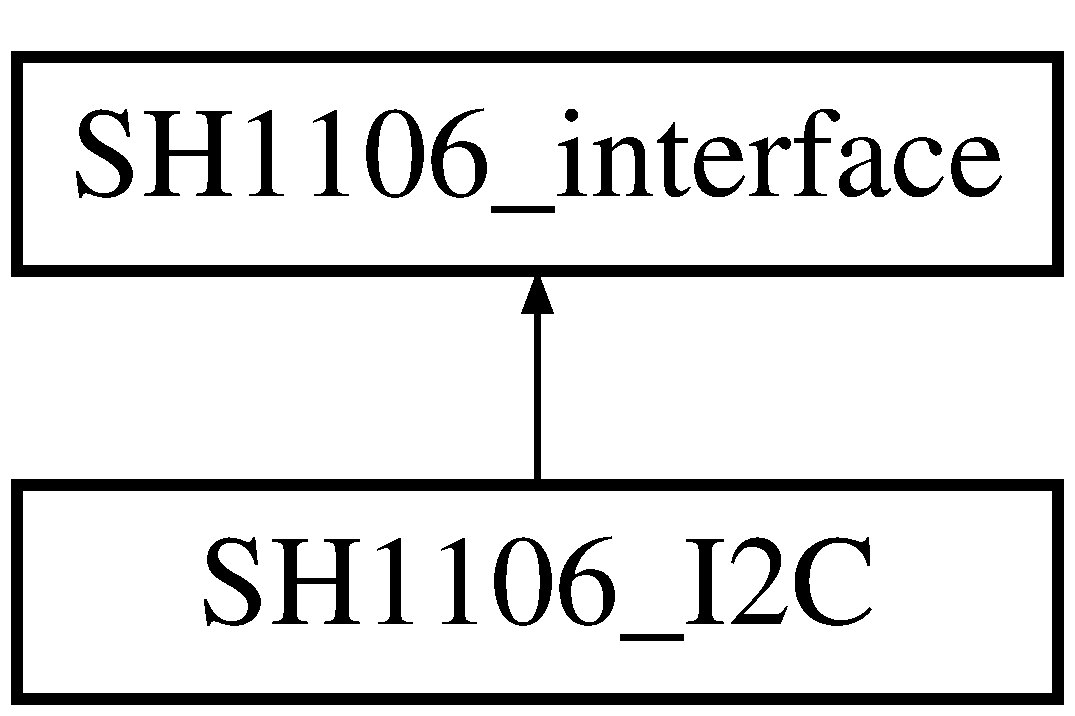
\includegraphics[height=2.000000cm]{class_s_h1106___i2_c}
\end{center}
\end{figure}
\subsection*{Public Member Functions}
\begin{DoxyCompactItemize}
\item 
\textbf{ S\+H1106\+\_\+\+I2C} (uint8\+\_\+t address=0x78, bool use\+Internal\+Pullup=true, uint32\+\_\+t frequency=100000)
\begin{DoxyCompactList}\small\item\em Constructor. \end{DoxyCompactList}\item 
void \textbf{ init} ()
\begin{DoxyCompactList}\small\item\em Initialize the i2c interface. \end{DoxyCompactList}\item 
bool \textbf{ check\+Connection} ()
\begin{DoxyCompactList}\small\item\em Returns true if the device at {\ttfamily address} sends an A\+CK on request. \end{DoxyCompactList}\item 
void \textbf{ send\+Command} (uint8\+\_\+t command)
\begin{DoxyCompactList}\small\item\em Send a command to the S\+H1106. \end{DoxyCompactList}\item 
void \textbf{ write\+R\+AM} (const uint8\+\_\+t data[$\,$], uint8\+\_\+t length)
\begin{DoxyCompactList}\small\item\em Write an array of data into the R\+AM of the S\+H1106 chip. \end{DoxyCompactList}\item 
void \textbf{ write\+R\+AM} (const uint8\+\_\+t data)
\begin{DoxyCompactList}\small\item\em Write a byte of data into the R\+AM of the S\+H1106 chip. \end{DoxyCompactList}\item 
bool \textbf{ is\+Enabled} ()
\begin{DoxyCompactList}\small\item\em Check whether the display is on or off. \end{DoxyCompactList}\item 
bool \textbf{ is\+Busy} ()
\begin{DoxyCompactList}\small\item\em Check whether the device is busy (i.\+e. it is executing a command) \end{DoxyCompactList}\end{DoxyCompactItemize}


\subsection{Detailed Description}
I2C interface implementation class This class allows to communicate with an S\+H1106 through i2c interface. 

This class provides low level i2c functions specific to the A\+Tmega328 microcontroller (like {\ttfamily \doxyref{init()}{p.}{class_s_h1106___i2_c_ae6c5529336068137a1060e120204c344}} and {\ttfamily start()}) as well as higher level functions that match S\+H1106 requirements (e.\+g. {\ttfamily \doxyref{send\+Command()}{p.}{class_s_h1106___i2_c_a118ff2bd4a7fc36ed9ece89306c60540}} and {\ttfamily control\+Byte()}).

The public functions are defined in the \doxyref{S\+H1106\+\_\+interface}{p.}{class_s_h1106__interface} abstract class. 

Definition at line 73 of file S\+H1106\+\_\+interfaces.\+hpp.



\subsection{Constructor \& Destructor Documentation}
\mbox{\label{class_s_h1106___i2_c_a64b034b97942eb6d72f5ea9b7afbb8db}} 
\index{S\+H1106\+\_\+\+I2C@{S\+H1106\+\_\+\+I2C}!S\+H1106\+\_\+\+I2C@{S\+H1106\+\_\+\+I2C}}
\index{S\+H1106\+\_\+\+I2C@{S\+H1106\+\_\+\+I2C}!S\+H1106\+\_\+\+I2C@{S\+H1106\+\_\+\+I2C}}
\subsubsection{S\+H1106\+\_\+\+I2\+C()}
{\footnotesize\ttfamily S\+H1106\+\_\+\+I2\+C\+::\+S\+H1106\+\_\+\+I2C (\begin{DoxyParamCaption}\item[{uint8\+\_\+t}]{address = {\ttfamily 0x78},  }\item[{bool}]{use\+Internal\+Pullup = {\ttfamily true},  }\item[{uint32\+\_\+t}]{frequency = {\ttfamily 100000} }\end{DoxyParamCaption})}



Constructor. 


\begin{DoxyParams}{Parameters}
{\em address} & Display I2C address [default\+: 0x78] \\
\hline
{\em use\+Internal\+Pullup} & Use A\+Tmega internal pullups as I2C bus pullup resistors [default\+: true] \\
\hline
{\em frequency} & I2C bus frequency [default\+: 100000] i \\
\hline
\end{DoxyParams}


Definition at line 10 of file S\+H1106\+\_\+\+I2\+C.\+cpp.



\subsection{Member Function Documentation}
\mbox{\label{class_s_h1106___i2_c_ae6c5529336068137a1060e120204c344}} 
\index{S\+H1106\+\_\+\+I2C@{S\+H1106\+\_\+\+I2C}!init@{init}}
\index{init@{init}!S\+H1106\+\_\+\+I2C@{S\+H1106\+\_\+\+I2C}}
\subsubsection{init()}
{\footnotesize\ttfamily void S\+H1106\+\_\+\+I2\+C\+::init (\begin{DoxyParamCaption}{ }\end{DoxyParamCaption})\hspace{0.3cm}{\ttfamily [virtual]}}



Initialize the i2c interface. 



Implements \textbf{ S\+H1106\+\_\+interface} \doxyref{}{p.}{class_s_h1106__interface_ac47fbd90dbd95e0ad39c19e0913a4a0a}.



Definition at line 19 of file S\+H1106\+\_\+\+I2\+C.\+cpp.

\mbox{\label{class_s_h1106___i2_c_a077880b268efac4f8e77af1864d3eac4}} 
\index{S\+H1106\+\_\+\+I2C@{S\+H1106\+\_\+\+I2C}!check\+Connection@{check\+Connection}}
\index{check\+Connection@{check\+Connection}!S\+H1106\+\_\+\+I2C@{S\+H1106\+\_\+\+I2C}}
\subsubsection{check\+Connection()}
{\footnotesize\ttfamily bool S\+H1106\+\_\+\+I2\+C\+::check\+Connection (\begin{DoxyParamCaption}{ }\end{DoxyParamCaption})\hspace{0.3cm}{\ttfamily [virtual]}}



Returns true if the device at {\ttfamily address} sends an A\+CK on request. 



Implements \textbf{ S\+H1106\+\_\+interface} \doxyref{}{p.}{class_s_h1106__interface_a2ff24f7c29cbb1eda6e61c448f405708}.



Definition at line 36 of file S\+H1106\+\_\+\+I2\+C.\+cpp.

\mbox{\label{class_s_h1106___i2_c_a118ff2bd4a7fc36ed9ece89306c60540}} 
\index{S\+H1106\+\_\+\+I2C@{S\+H1106\+\_\+\+I2C}!send\+Command@{send\+Command}}
\index{send\+Command@{send\+Command}!S\+H1106\+\_\+\+I2C@{S\+H1106\+\_\+\+I2C}}
\subsubsection{send\+Command()}
{\footnotesize\ttfamily void S\+H1106\+\_\+\+I2\+C\+::send\+Command (\begin{DoxyParamCaption}\item[{uint8\+\_\+t}]{command }\end{DoxyParamCaption})\hspace{0.3cm}{\ttfamily [virtual]}}



Send a command to the S\+H1106. 

\begin{DoxyNote}{Note}
This function contains a full i2c transaction (from start to stop) 
\end{DoxyNote}

\begin{DoxyParams}{Parameters}
{\em command} & single byte that will be interpreted as a command \\
\hline
\end{DoxyParams}


Implements \textbf{ S\+H1106\+\_\+interface} \doxyref{}{p.}{class_s_h1106__interface_a22f10681d2b53b39bba4307e5c6c6efa}.



Definition at line 51 of file S\+H1106\+\_\+\+I2\+C.\+cpp.

\mbox{\label{class_s_h1106___i2_c_a9fba08e53f1a6ca36c8dc4faef4f949d}} 
\index{S\+H1106\+\_\+\+I2C@{S\+H1106\+\_\+\+I2C}!write\+R\+AM@{write\+R\+AM}}
\index{write\+R\+AM@{write\+R\+AM}!S\+H1106\+\_\+\+I2C@{S\+H1106\+\_\+\+I2C}}
\subsubsection{write\+R\+A\+M()\hspace{0.1cm}{\footnotesize\ttfamily [1/2]}}
{\footnotesize\ttfamily void S\+H1106\+\_\+\+I2\+C\+::write\+R\+AM (\begin{DoxyParamCaption}\item[{const uint8\+\_\+t}]{data[$\,$],  }\item[{uint8\+\_\+t}]{length }\end{DoxyParamCaption})\hspace{0.3cm}{\ttfamily [virtual]}}



Write an array of data into the R\+AM of the S\+H1106 chip. 

\begin{DoxyNote}{Note}
This function contains one single i2c transaction 
\end{DoxyNote}

\begin{DoxyParams}{Parameters}
{\em data} & array of bytes to be sent \\
\hline
{\em length} & length of the data array \\
\hline
\end{DoxyParams}


Implements \textbf{ S\+H1106\+\_\+interface} \doxyref{}{p.}{class_s_h1106__interface_ae987e7ec271292ce4b8c39b0d2ba2d5e}.



Definition at line 60 of file S\+H1106\+\_\+\+I2\+C.\+cpp.

\mbox{\label{class_s_h1106___i2_c_af4e00228a3e7c11496de302f10edc6ae}} 
\index{S\+H1106\+\_\+\+I2C@{S\+H1106\+\_\+\+I2C}!write\+R\+AM@{write\+R\+AM}}
\index{write\+R\+AM@{write\+R\+AM}!S\+H1106\+\_\+\+I2C@{S\+H1106\+\_\+\+I2C}}
\subsubsection{write\+R\+A\+M()\hspace{0.1cm}{\footnotesize\ttfamily [2/2]}}
{\footnotesize\ttfamily void S\+H1106\+\_\+\+I2\+C\+::write\+R\+AM (\begin{DoxyParamCaption}\item[{const uint8\+\_\+t}]{data }\end{DoxyParamCaption})\hspace{0.3cm}{\ttfamily [virtual]}}



Write a byte of data into the R\+AM of the S\+H1106 chip. 

\begin{DoxyNote}{Note}
This function contains one single i2c transaction 
\end{DoxyNote}

\begin{DoxyParams}{Parameters}
{\em data} & byte to send \\
\hline
\end{DoxyParams}


Implements \textbf{ S\+H1106\+\_\+interface} \doxyref{}{p.}{class_s_h1106__interface_a20725a0fa95fd6849333d2605ca3b090}.



Definition at line 70 of file S\+H1106\+\_\+\+I2\+C.\+cpp.

\mbox{\label{class_s_h1106___i2_c_af5bc8c96f70163d6215423c07f94da49}} 
\index{S\+H1106\+\_\+\+I2C@{S\+H1106\+\_\+\+I2C}!is\+Enabled@{is\+Enabled}}
\index{is\+Enabled@{is\+Enabled}!S\+H1106\+\_\+\+I2C@{S\+H1106\+\_\+\+I2C}}
\subsubsection{is\+Enabled()}
{\footnotesize\ttfamily bool S\+H1106\+\_\+\+I2\+C\+::is\+Enabled (\begin{DoxyParamCaption}{ }\end{DoxyParamCaption})\hspace{0.3cm}{\ttfamily [virtual]}}



Check whether the display is on or off. 



Implements \textbf{ S\+H1106\+\_\+interface} \doxyref{}{p.}{class_s_h1106__interface_a7d1baf8c3e41ff19f05b03a38b1eca7a}.



Definition at line 80 of file S\+H1106\+\_\+\+I2\+C.\+cpp.

\mbox{\label{class_s_h1106___i2_c_acec7469a16d4f9ac2d0cac76eb75c544}} 
\index{S\+H1106\+\_\+\+I2C@{S\+H1106\+\_\+\+I2C}!is\+Busy@{is\+Busy}}
\index{is\+Busy@{is\+Busy}!S\+H1106\+\_\+\+I2C@{S\+H1106\+\_\+\+I2C}}
\subsubsection{is\+Busy()}
{\footnotesize\ttfamily bool S\+H1106\+\_\+\+I2\+C\+::is\+Busy (\begin{DoxyParamCaption}{ }\end{DoxyParamCaption})\hspace{0.3cm}{\ttfamily [virtual]}}



Check whether the device is busy (i.\+e. it is executing a command) 



Implements \textbf{ S\+H1106\+\_\+interface} \doxyref{}{p.}{class_s_h1106__interface_a9ff43dbad062c27049498497324d958e}.



Definition at line 89 of file S\+H1106\+\_\+\+I2\+C.\+cpp.



The documentation for this class was generated from the following files\+:\begin{DoxyCompactItemize}
\item 
/\+Users/noe/\+Documents/\+Robot/\+Librerie/\+S\+H1106/\+S\+H1106/S\+H1106\+\_\+interfaces.\+hpp\item 
/\+Users/noe/\+Documents/\+Robot/\+Librerie/\+S\+H1106/\+S\+H1106/S\+H1106\+\_\+\+I2\+C.\+cpp\end{DoxyCompactItemize}

\section{S\+H1106\+\_\+interface Class Reference}
\label{class_s_h1106__interface}\index{S\+H1106\+\_\+interface@{S\+H1106\+\_\+interface}}


Abstract class to describe any interface to communicate with S\+H1106.  




{\ttfamily \#include $<$S\+H1106\+\_\+interfaces.\+hpp$>$}

Inheritance diagram for S\+H1106\+\_\+interface\+:\begin{figure}[H]
\begin{center}
\leavevmode
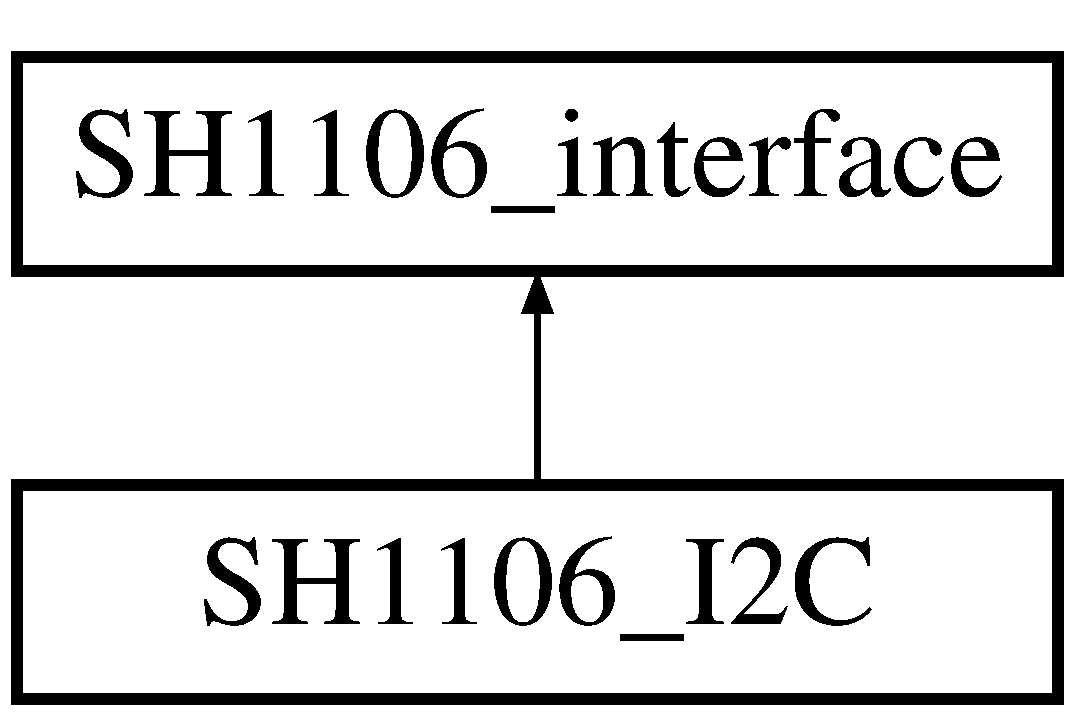
\includegraphics[height=2.000000cm]{class_s_h1106__interface}
\end{center}
\end{figure}
\subsection*{Public Member Functions}
\begin{DoxyCompactItemize}
\item 
virtual void \textbf{ init} ()=0
\begin{DoxyCompactList}\small\item\em Initialize the communication interface. \end{DoxyCompactList}\item 
virtual bool \textbf{ check\+Connection} ()=0
\begin{DoxyCompactList}\small\item\em Returns true if a device is connected (possibly check whether it is an S\+H1106) \end{DoxyCompactList}\item 
virtual void \textbf{ send\+Command} (uint8\+\_\+t command)=0
\begin{DoxyCompactList}\small\item\em Send a command to the S\+H1106. \end{DoxyCompactList}\item 
virtual void \textbf{ write\+R\+AM} (const uint8\+\_\+t data[$\,$], uint8\+\_\+t length)=0
\begin{DoxyCompactList}\small\item\em Write an array of data into the R\+AM of the S\+H1106. \end{DoxyCompactList}\item 
virtual void \textbf{ write\+R\+AM} (const uint8\+\_\+t data)=0
\begin{DoxyCompactList}\small\item\em Write a byte of data into the R\+AM of the S\+H1106. \end{DoxyCompactList}\item 
virtual bool \textbf{ is\+Enabled} ()=0
\begin{DoxyCompactList}\small\item\em Check whether the display is on or off. \end{DoxyCompactList}\item 
virtual bool \textbf{ is\+Busy} ()=0
\begin{DoxyCompactList}\small\item\em Check whether the device is busy (i.\+e. it is executing a command) \end{DoxyCompactList}\end{DoxyCompactItemize}


\subsection{Detailed Description}
Abstract class to describe any interface to communicate with S\+H1106. 

The S\+H1106 O\+L\+ED Controller features many different communication interfaces\+:

8-\/bit 6800-\/series parallel 8-\/bit 8080-\/series parallel 3-\/wire S\+PI 4-\/wire S\+PI I2C

This library was originally intended designed to use i2c, but this interface should not be hardcoded in the higher level functions. Hence this abstract class will be used in all higher level classes and methods declaration instead of an interface-\/specific \char`\"{}concrete\char`\"{} class. This way changing the communication interface will only require a single change in the constructor of the \char`\"{}next level\char`\"{} class, i.\+e. S\+H1106 (by passing e.\+g. an S\+H1106\+\_\+3\+S\+PI object instead of an \doxyref{S\+H1106\+\_\+\+I2C}{p.}{class_s_h1106___i2_c} one). If there is not any class for the desider interface yet, the user will need to write a class derived from this one. 

Definition at line 36 of file S\+H1106\+\_\+interfaces.\+hpp.



\subsection{Member Function Documentation}
\mbox{\label{class_s_h1106__interface_ac47fbd90dbd95e0ad39c19e0913a4a0a}} 
\index{S\+H1106\+\_\+interface@{S\+H1106\+\_\+interface}!init@{init}}
\index{init@{init}!S\+H1106\+\_\+interface@{S\+H1106\+\_\+interface}}
\subsubsection{init()}
{\footnotesize\ttfamily virtual void S\+H1106\+\_\+interface\+::init (\begin{DoxyParamCaption}{ }\end{DoxyParamCaption})\hspace{0.3cm}{\ttfamily [pure virtual]}}



Initialize the communication interface. 



Implemented in \textbf{ S\+H1106\+\_\+\+I2C} \doxyref{}{p.}{class_s_h1106___i2_c_ae6c5529336068137a1060e120204c344}.

\mbox{\label{class_s_h1106__interface_a2ff24f7c29cbb1eda6e61c448f405708}} 
\index{S\+H1106\+\_\+interface@{S\+H1106\+\_\+interface}!check\+Connection@{check\+Connection}}
\index{check\+Connection@{check\+Connection}!S\+H1106\+\_\+interface@{S\+H1106\+\_\+interface}}
\subsubsection{check\+Connection()}
{\footnotesize\ttfamily virtual bool S\+H1106\+\_\+interface\+::check\+Connection (\begin{DoxyParamCaption}{ }\end{DoxyParamCaption})\hspace{0.3cm}{\ttfamily [pure virtual]}}



Returns true if a device is connected (possibly check whether it is an S\+H1106) 



Implemented in \textbf{ S\+H1106\+\_\+\+I2C} \doxyref{}{p.}{class_s_h1106___i2_c_a077880b268efac4f8e77af1864d3eac4}.

\mbox{\label{class_s_h1106__interface_a22f10681d2b53b39bba4307e5c6c6efa}} 
\index{S\+H1106\+\_\+interface@{S\+H1106\+\_\+interface}!send\+Command@{send\+Command}}
\index{send\+Command@{send\+Command}!S\+H1106\+\_\+interface@{S\+H1106\+\_\+interface}}
\subsubsection{send\+Command()}
{\footnotesize\ttfamily virtual void S\+H1106\+\_\+interface\+::send\+Command (\begin{DoxyParamCaption}\item[{uint8\+\_\+t}]{command }\end{DoxyParamCaption})\hspace{0.3cm}{\ttfamily [pure virtual]}}



Send a command to the S\+H1106. 



Implemented in \textbf{ S\+H1106\+\_\+\+I2C} \doxyref{}{p.}{class_s_h1106___i2_c_a118ff2bd4a7fc36ed9ece89306c60540}.

\mbox{\label{class_s_h1106__interface_ae987e7ec271292ce4b8c39b0d2ba2d5e}} 
\index{S\+H1106\+\_\+interface@{S\+H1106\+\_\+interface}!write\+R\+AM@{write\+R\+AM}}
\index{write\+R\+AM@{write\+R\+AM}!S\+H1106\+\_\+interface@{S\+H1106\+\_\+interface}}
\subsubsection{write\+R\+A\+M()\hspace{0.1cm}{\footnotesize\ttfamily [1/2]}}
{\footnotesize\ttfamily virtual void S\+H1106\+\_\+interface\+::write\+R\+AM (\begin{DoxyParamCaption}\item[{const uint8\+\_\+t}]{data[$\,$],  }\item[{uint8\+\_\+t}]{length }\end{DoxyParamCaption})\hspace{0.3cm}{\ttfamily [pure virtual]}}



Write an array of data into the R\+AM of the S\+H1106. 



Implemented in \textbf{ S\+H1106\+\_\+\+I2C} \doxyref{}{p.}{class_s_h1106___i2_c_a9fba08e53f1a6ca36c8dc4faef4f949d}.

\mbox{\label{class_s_h1106__interface_a20725a0fa95fd6849333d2605ca3b090}} 
\index{S\+H1106\+\_\+interface@{S\+H1106\+\_\+interface}!write\+R\+AM@{write\+R\+AM}}
\index{write\+R\+AM@{write\+R\+AM}!S\+H1106\+\_\+interface@{S\+H1106\+\_\+interface}}
\subsubsection{write\+R\+A\+M()\hspace{0.1cm}{\footnotesize\ttfamily [2/2]}}
{\footnotesize\ttfamily virtual void S\+H1106\+\_\+interface\+::write\+R\+AM (\begin{DoxyParamCaption}\item[{const uint8\+\_\+t}]{data }\end{DoxyParamCaption})\hspace{0.3cm}{\ttfamily [pure virtual]}}



Write a byte of data into the R\+AM of the S\+H1106. 



Implemented in \textbf{ S\+H1106\+\_\+\+I2C} \doxyref{}{p.}{class_s_h1106___i2_c_af4e00228a3e7c11496de302f10edc6ae}.

\mbox{\label{class_s_h1106__interface_a7d1baf8c3e41ff19f05b03a38b1eca7a}} 
\index{S\+H1106\+\_\+interface@{S\+H1106\+\_\+interface}!is\+Enabled@{is\+Enabled}}
\index{is\+Enabled@{is\+Enabled}!S\+H1106\+\_\+interface@{S\+H1106\+\_\+interface}}
\subsubsection{is\+Enabled()}
{\footnotesize\ttfamily virtual bool S\+H1106\+\_\+interface\+::is\+Enabled (\begin{DoxyParamCaption}{ }\end{DoxyParamCaption})\hspace{0.3cm}{\ttfamily [pure virtual]}}



Check whether the display is on or off. 



Implemented in \textbf{ S\+H1106\+\_\+\+I2C} \doxyref{}{p.}{class_s_h1106___i2_c_af5bc8c96f70163d6215423c07f94da49}.

\mbox{\label{class_s_h1106__interface_a9ff43dbad062c27049498497324d958e}} 
\index{S\+H1106\+\_\+interface@{S\+H1106\+\_\+interface}!is\+Busy@{is\+Busy}}
\index{is\+Busy@{is\+Busy}!S\+H1106\+\_\+interface@{S\+H1106\+\_\+interface}}
\subsubsection{is\+Busy()}
{\footnotesize\ttfamily virtual bool S\+H1106\+\_\+interface\+::is\+Busy (\begin{DoxyParamCaption}{ }\end{DoxyParamCaption})\hspace{0.3cm}{\ttfamily [pure virtual]}}



Check whether the device is busy (i.\+e. it is executing a command) 



Implemented in \textbf{ S\+H1106\+\_\+\+I2C} \doxyref{}{p.}{class_s_h1106___i2_c_acec7469a16d4f9ac2d0cac76eb75c544}.



The documentation for this class was generated from the following file\+:\begin{DoxyCompactItemize}
\item 
/\+Users/noe/\+Documents/\+Robot/\+Librerie/\+S\+H1106/\+S\+H1106/S\+H1106\+\_\+interfaces.\+hpp\end{DoxyCompactItemize}

%--- End generated contents ---

% Index
\backmatter
\newpage
\phantomsection
\clearemptydoublepage
\addcontentsline{toc}{chapter}{Index}
\printindex

\end{document}
